\section{Results}

This section reports the main results that are proved to be robust by our analysis. The estimates are grouped into player-game effects, tournament participation effects, move-level mechanisms, and style results. Detailed stargazer-generated tables are included in the project folder \texttt{tables/}; compact versions are shown below for readability.

\begin{figure}[H]
\centering
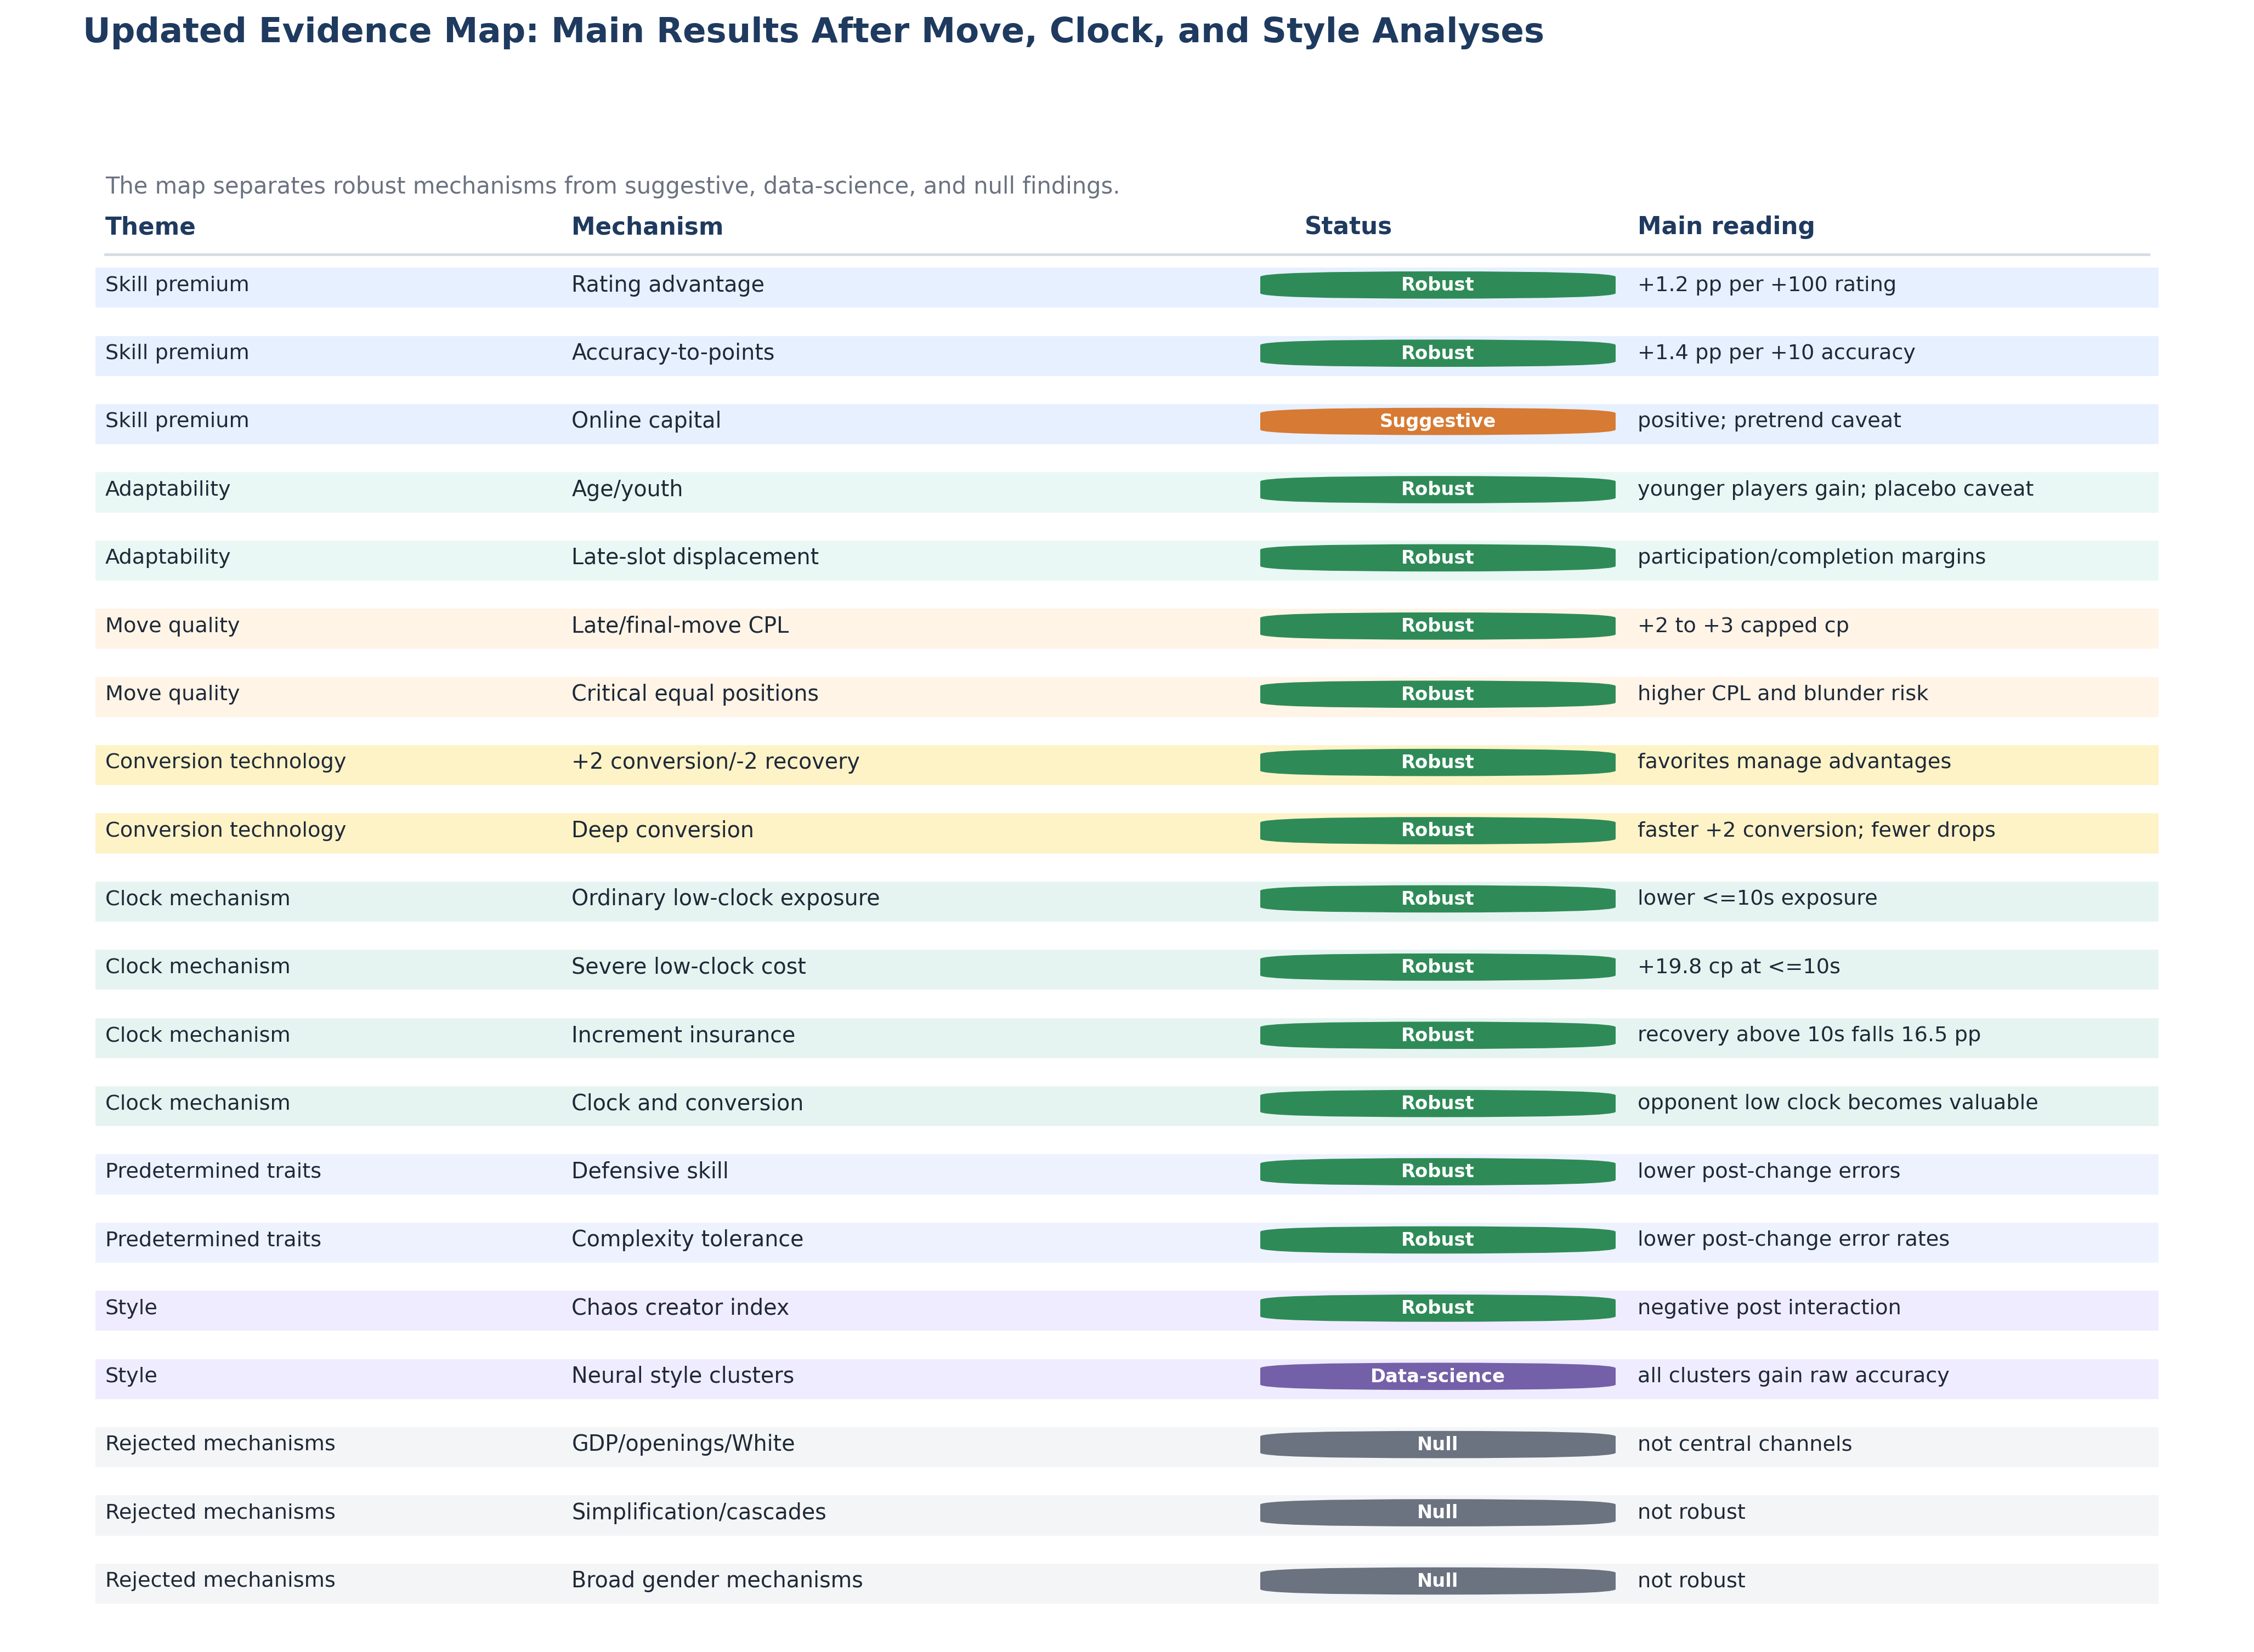
\includegraphics[width=\textwidth]{figures/figure10_clean_outline_evidence_map.png}
\caption{Key findings after the game-level, move-level, clock, and style analyses.}
\label{fig:evidence-map}
\end{figure}

\subsection{Relative Skill Became More Valuable}

The strongest game-level result is that the post-change format increased the return to rating advantage. Table \ref{tab:main-game-results} summarizes the baseline treatment interactions. The coefficient on \(\text{Post} \times \text{RatingDiff100}\) is 0.0119 in the clean thesis table and 0.0122 in the validation report. The interpretation is direct: after the switch to 5+0, a 100-point rating edge was associated with about 1.2 additional percentage points of score result.

\begin{table}[H]
\centering
\caption{Baseline Game-Level Treatment Effects}
\label{tab:main-game-results}
\begin{adjustbox}{max width=\textwidth}
\begin{tabular}{llrrrrl}
\toprule
Result & Outcome & Estimate & SE & p-value & N & Unit \\
\midrule
Relative skill return & Player result & 0.0119 & 0.0010 & \(<0.001\) & 1,335,043 & Per +100 rating advantage \\
Accuracy-to-points conversion & Player result & 0.0141 & 0.0023 & \(<0.001\) & 1,284,771 & Per +10 accuracy points \\
Online-platform capital & Player result & 0.0093 & 0.0013 & \(<0.001\) & 1,315,216 & Per +100 Chess.com-over-classical rating \\
Age heterogeneity & Player result & -0.0145 & 0.0016 & \(<0.001\) & 1,335,043 & Per +10 years of age \\
\bottomrule
\end{tabular}
\end{adjustbox}
\end{table}

The magnitude is economically meaningful. A 200-point favorite gained about 2.4 additional percentage points of expected score after the reform. Moving from the 25th to the 75th percentile of rating difference corresponds to about 5.5 percentage points in score share. Win/loss decomposition shows that the effect is not only a draw-margin change. The probability of winning increases by about 1.3 percentage points per 100 rating points, while the probability of losing falls by about 1.2 percentage points. Draw probability changes little.

Table \ref{tab:rating-robustness} shows the main robustness checks. The coefficient remains positive and close in magnitude when early rounds are excluded, when the sample is restricted to a twelve-month window around the reform, when only balanced players are used, and when paired-game fixed effects are added. The paired-game fixed-effect estimate is smaller, about 0.0095, but it remains economically meaningful.

\begin{table}[H]
\centering
\caption{Robustness of the Rating-Advantage Result}
\label{tab:rating-robustness}
\begin{tabular}{lrrl}
\toprule
Specification & Estimate & SE & Interpretation \\
\midrule
Event FE, rounds \(>1\) & 0.0122 & 0.0010 & Main design \\
Exclude rounds 1 and 2 & 0.0139 & 0.0011 & Similar after removing early Swiss noise \\
\(\pm\)12 month window & 0.0134 & 0.0015 & Similar near the reform \\
Balanced players only & 0.0117 & 0.0011 & Similar among repeat players \\
Paired-game FE & 0.0095 & 0.0012 & Same-game comparison \\
Placebo-grid mean & 0.0017 & -- & Much smaller than actual estimate \\
\bottomrule
\end{tabular}
\end{table}

Figure \ref{fig:rating-robustness-advanced} presents the same robustness pattern graphically. The placebo-grid estimate is close to zero and its confidence interval lies far below the estimates from the main designs.

\begin{figure}[H]
\centering
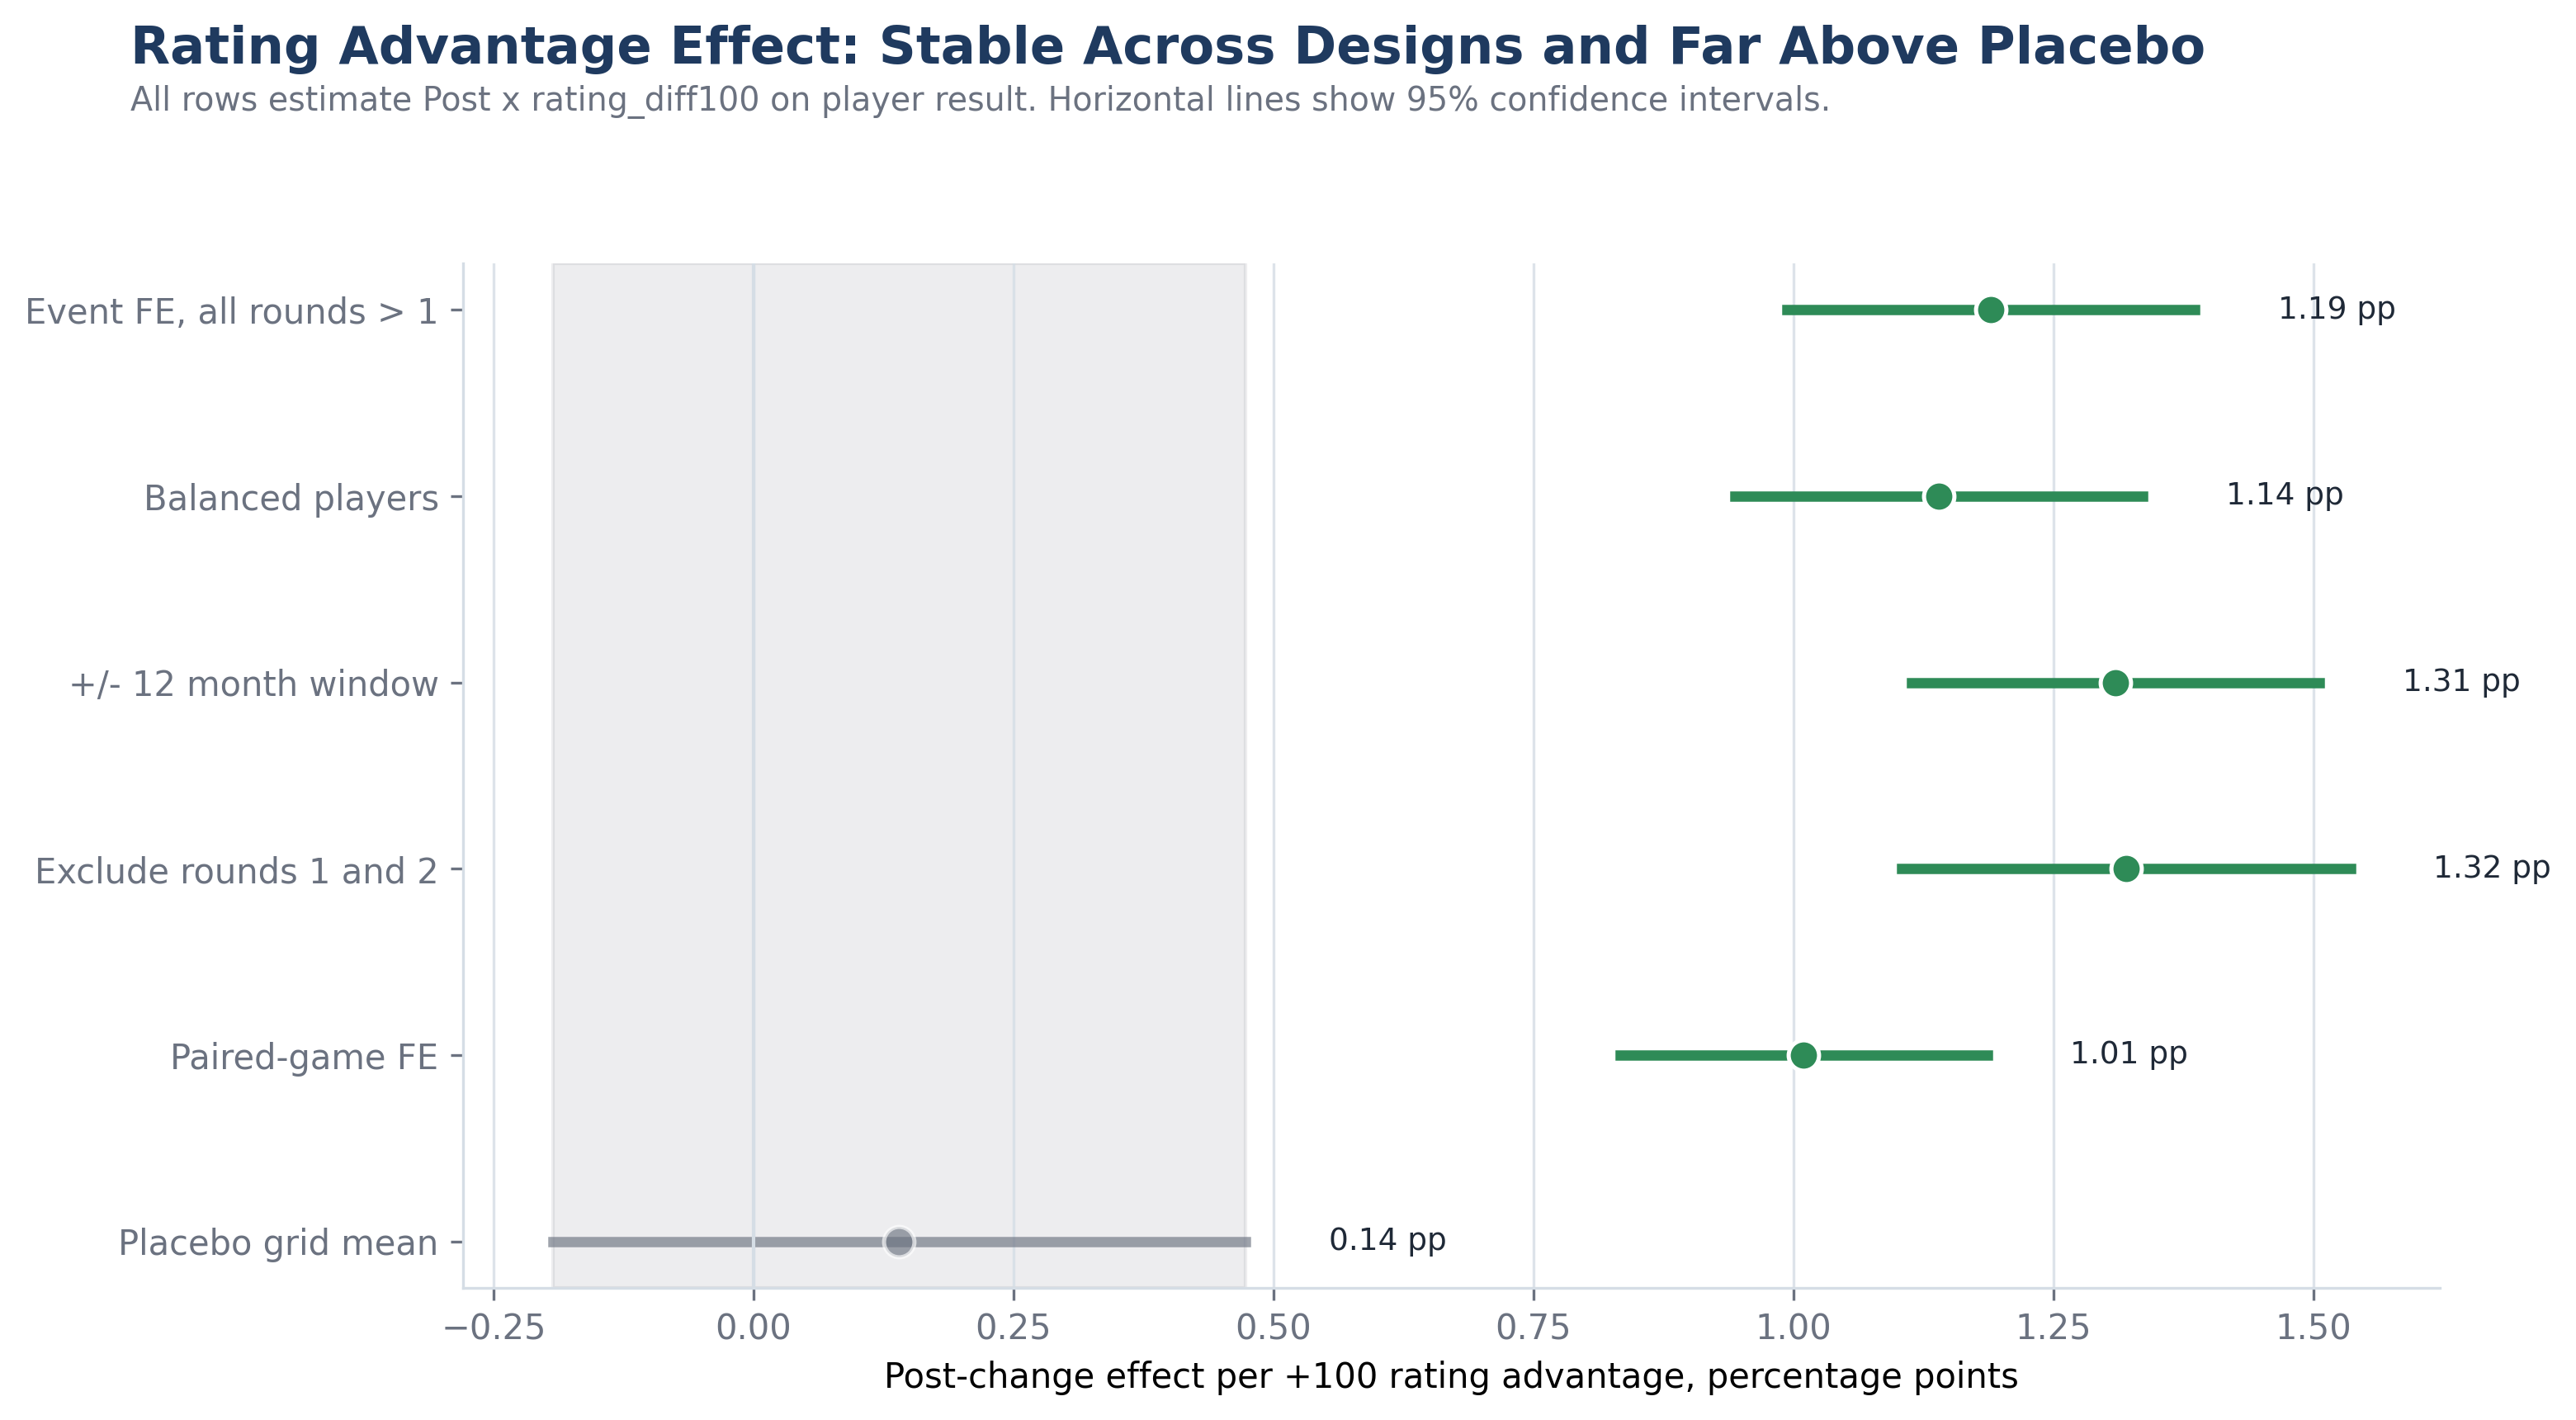
\includegraphics[width=0.92\textwidth]{figures/figure8_rating_robustness_advanced.png}
\caption{Coefficient plot for the rating-advantage result across robustness designs.}
\label{fig:rating-robustness-advanced}
\end{figure}

The placebo evidence is especially important. Across fake pre-reform cutoffs, the mean placebo coefficient is around 0.0017 and the 90th percentile is around 0.0031, far below the actual estimate. The linear pretrend in the pre-period is small and negative, not positive. Figure \ref{fig:rating-event-study} shows the event-study pattern for the rating-difference return and connects it to the newly available clock data. The post-change coefficients rise relative to the pre-change reference period, while the pre-period does not display a comparable upward movement. The clock panels show that ordinary low-clock exposure fell after the reform, but the centipawn-loss penalty of severe low-clock states became much larger under 5+0.

\begin{figure}[H]
\centering
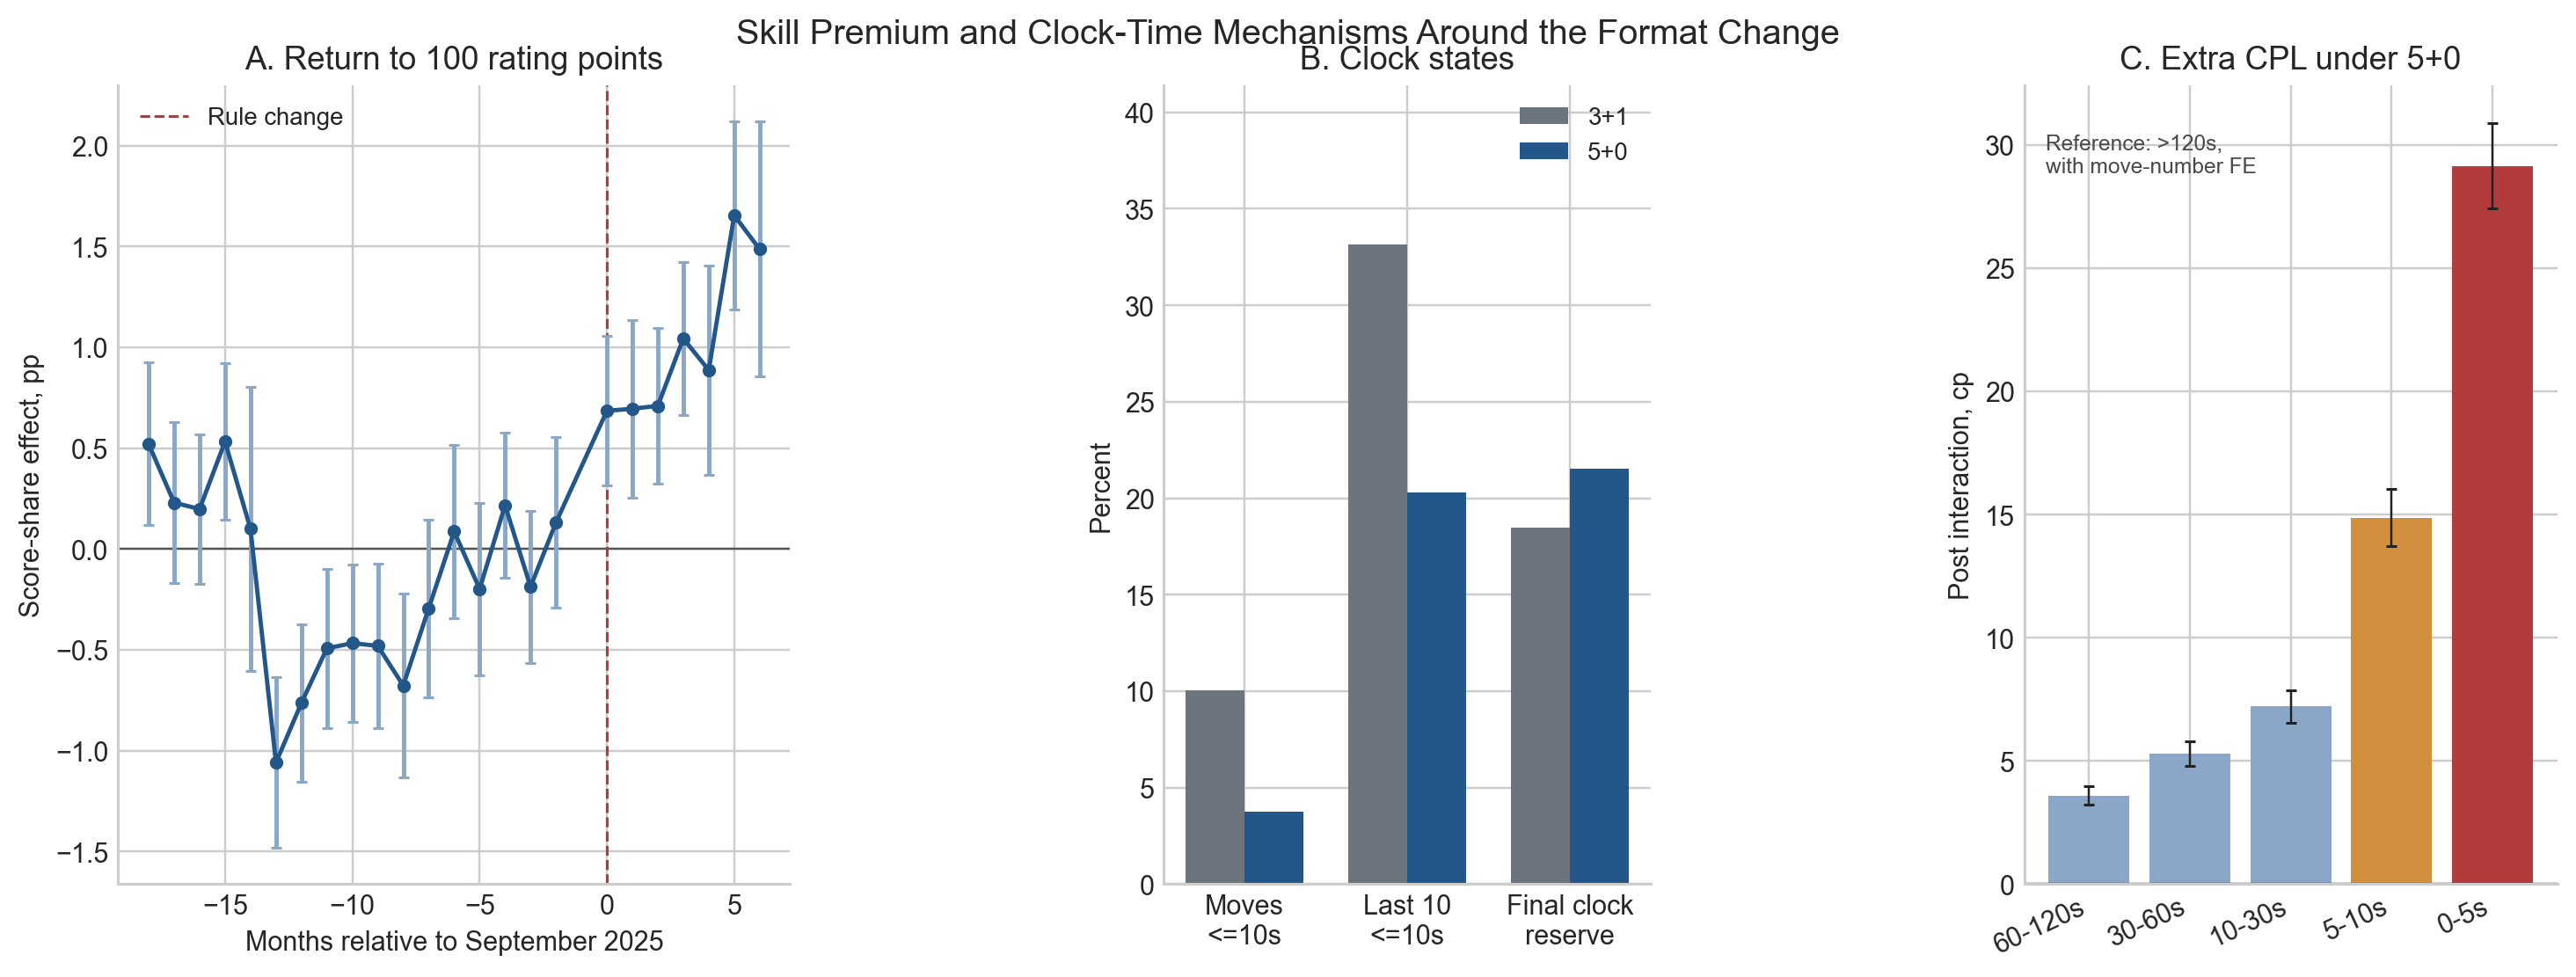
\includegraphics[width=\textwidth]{figures/figure1_rating_diff_event_study.png}
\caption{Rating advantage and clock-time mechanisms around the reform. Panel A reports the event-study return to a 100-point rating advantage. Panel B compares clock exposure and final clock reserve before and after the reform. Panel C reports post-change centipawn-loss interactions by remaining-clock bin, with move-number fixed effects.}
\label{fig:rating-event-study}
\end{figure}

This result is the cleanest evidence in the thesis. It shows that the new format did not primarily increase underdog randomness. Instead, conditional on playing, ex ante stronger players converted their rating advantage more effectively under 5+0.

\subsection{Accuracy Advantages Converted More Strongly into Points}

The production-function result is also strong, though it has a different interpretation. Accuracy is measured inside the game, so it should not be treated as a predetermined causal variable. It is better understood as a measure of the realized quality advantage in the game. The coefficient on \(\text{Post} \times \text{AccuracyDiff10}\) is 0.0141 in the compact thesis table and 0.0347 in the broader production-function battery. Both versions show the same pattern: after the reform, a given accuracy advantage translated into more score share.

In the broader battery, a 10-point accuracy advantage became worth about 3.5 additional percentage points of score share. The effect remains similar with paired-game fixed effects and when rounds 1 and 2 are excluded. The model using result over expected score also remains positive. Placebo estimates are smaller than the actual estimate, although there is evidence of a positive pretrend, so the safest wording is that the reform sharply amplified a pre-existing increase in accuracy-to-result conversion.

The interpretation is that 5+0 made the result more tightly connected to actual move quality. If one player outplayed the opponent by the same amount, that edge was more likely to become a full point or half-point advantage after the rule change. This complements the rating result: stronger players gained, and the mapping from realized quality to points became steeper.

Additional tests show that this production-function shift is not mainly a rating-favorite channel. The triple interaction \(\text{Post} \times \text{AccuracyDiff10} \times \text{RatingDiff100}\) is not statistically clear. The same is true for the online-capital triple interaction. Favorites gained, but not because the same accuracy edge became disproportionately more valuable only for favorites.

\subsection{Online-Platform Capital and Age Adaptability}

The online-platform result suggests that Chess.com-specific skill mattered more after the reform. Players whose Chess.com rating was high relative to classical rating gained about 0.9 to 1.1 percentage points per 100 rating points of online-over-classical advantage. The same broad pattern appears for Chess.com-over-FIDE blitz gaps. This is consistent with the idea that 5+0 online play rewards platform-specific human capital: mouse speed, interface fluency, premoves, practical no-increment experience, and comfort with the Chess.com playing environment.

This result is robust as an association, but it is not as clean as the rating-advantage result. Placebo and event-study checks suggest that returns to online specialization were already rising before September 2025. The most careful interpretation is therefore that the rule change reinforced an ongoing rise in the value of online-specific capital, rather than creating the whole effect from zero.

Age heterogeneity is statistically strong. The main player-game estimate is about -0.0145 per 10 years of age. Within-game age-gap comparisons are also negative: after the reform, older players performed worse relative to younger opponents in the same game. In games between young and old players, the post-change score shifted by about 2.3 percentage points toward the young player. The accuracy result is directionally similar, with older players losing about 0.15 accuracy points per additional decade.

\begin{figure}[H]
\centering
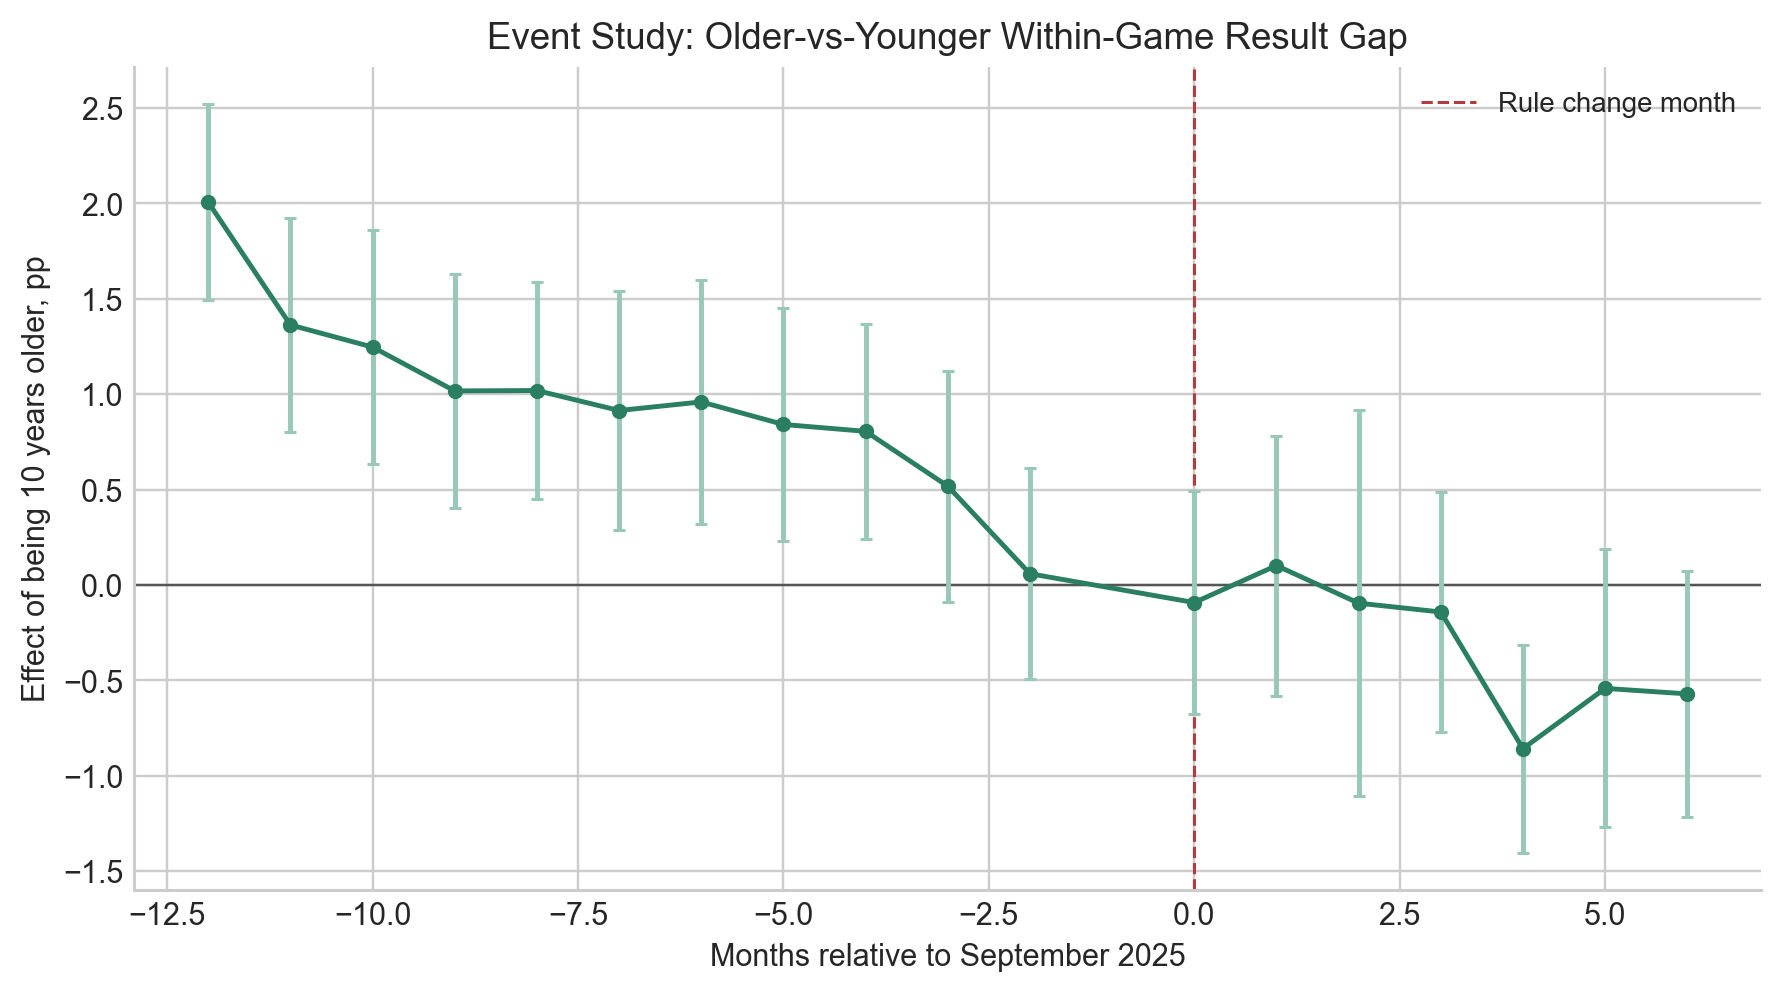
\includegraphics[width=0.90\textwidth]{figures/figure2_age_gap_event_study.png}
\caption{Event-study and coefficient pattern for the age-gap result.}
\label{fig:age-event-study}
\end{figure}

The caveat is that a September 2024 placebo cutoff also gives negative age effects, although smaller. For this reason, the thesis treats age as strong heterogeneity evidence and a plausible adaptability channel, not as a perfectly clean discontinuity. The most supported statement is descriptive: younger players gained relative to older players in the new format, and this pattern is visible in several within-player and within-game specifications.

\subsection{Time-Slot Displacement}

The reform removed the old late Titled Tuesday slot. Before the reform, the dataset contains 188 early-slot events and 187 late-slot events. After the reform, it contains 31 early-slot events and no late-slot events. This creates a second treatment margin: players who were late-slot regulars faced a larger schedule shock.

The time-slot evidence is strongest for participation and completion. Moving from a pure early-slot player to a pure late-slot player predicts a 13.3 percentage point lower probability of appearing after the reform and about 1.38 fewer post-reform tournaments out of 31 available. Conditional on returning, late regulars completed fewer rounds and had lower tournament score and rank. Table \ref{tab:timeslot} summarizes the main estimates.

\begin{table}[H]
\centering
\caption{Time-Slot Displacement Results}
\label{tab:timeslot}
\begin{adjustbox}{max width=\textwidth}
\begin{tabular}{llrrrl}
\toprule
Outcome & Treatment & Estimate & SE & p-value & Interpretation \\
\midrule
Any post-rule event & Pre late share & -0.133 & 0.018 & \(<0.001\) & Lower post participation \\
Number of post events & Pre late share & -1.376 & 0.163 & \(<0.001\) & Fewer post tournaments \\
Score after round 1 & Late regular & -0.0367 & 0.0094 & \(<0.001\) & Lower tournament score \\
Rank percentile & Late regular & -0.0397 & 0.0107 & \(<0.001\) & Worse final rank \\
Games after round 1 & Late regular & -0.0619 & 0.0145 & \(<0.001\) & Fewer games completed \\
Completed after round 1 & Late regular & -0.0741 & 0.0239 & 0.002 & Lower completion \\
Per-game result & Late regular & 0.0061 & 0.0095 & 0.522 & No clear game penalty \\
Per-game accuracy & Late regular & -0.097 & 0.143 & 0.500 & No clear accuracy penalty \\
\bottomrule
\end{tabular}
\end{adjustbox}
\end{table}

The important distinction is between tournament-level and game-level outcomes. Late regulars do worse in tournament score and rank because they participate less and complete fewer rounds. Conditional on sitting down to play a game, there is no clear evidence that they score worse or play less accurately. The schedule component therefore mainly affects selection and tournament completion.

\subsection{Field Composition, Pairing Structure, and Rank Movement}

The reform also changed the tournament environment. Event-level evidence shows that the field became smaller and more positively selected. Mean field rating rose by roughly 100 rating points in a raw interrupted-series model and by about 71 rating points when adding a calendar trend. Field size fell by roughly 97 players. These shifts matter because the post-change event is not simply the same population playing a different clock format.

Pairing structure also changed. Same-score pairings became less frequent, rating gaps narrowed, and pregame score gaps widened. Figure \ref{fig:rankmovement} shows rank movement by rating-advantage bin. The post-change tournament appears to reward rating advantage more strongly in final ranking as well as in individual game outcomes.

\begin{figure}[H]
\centering
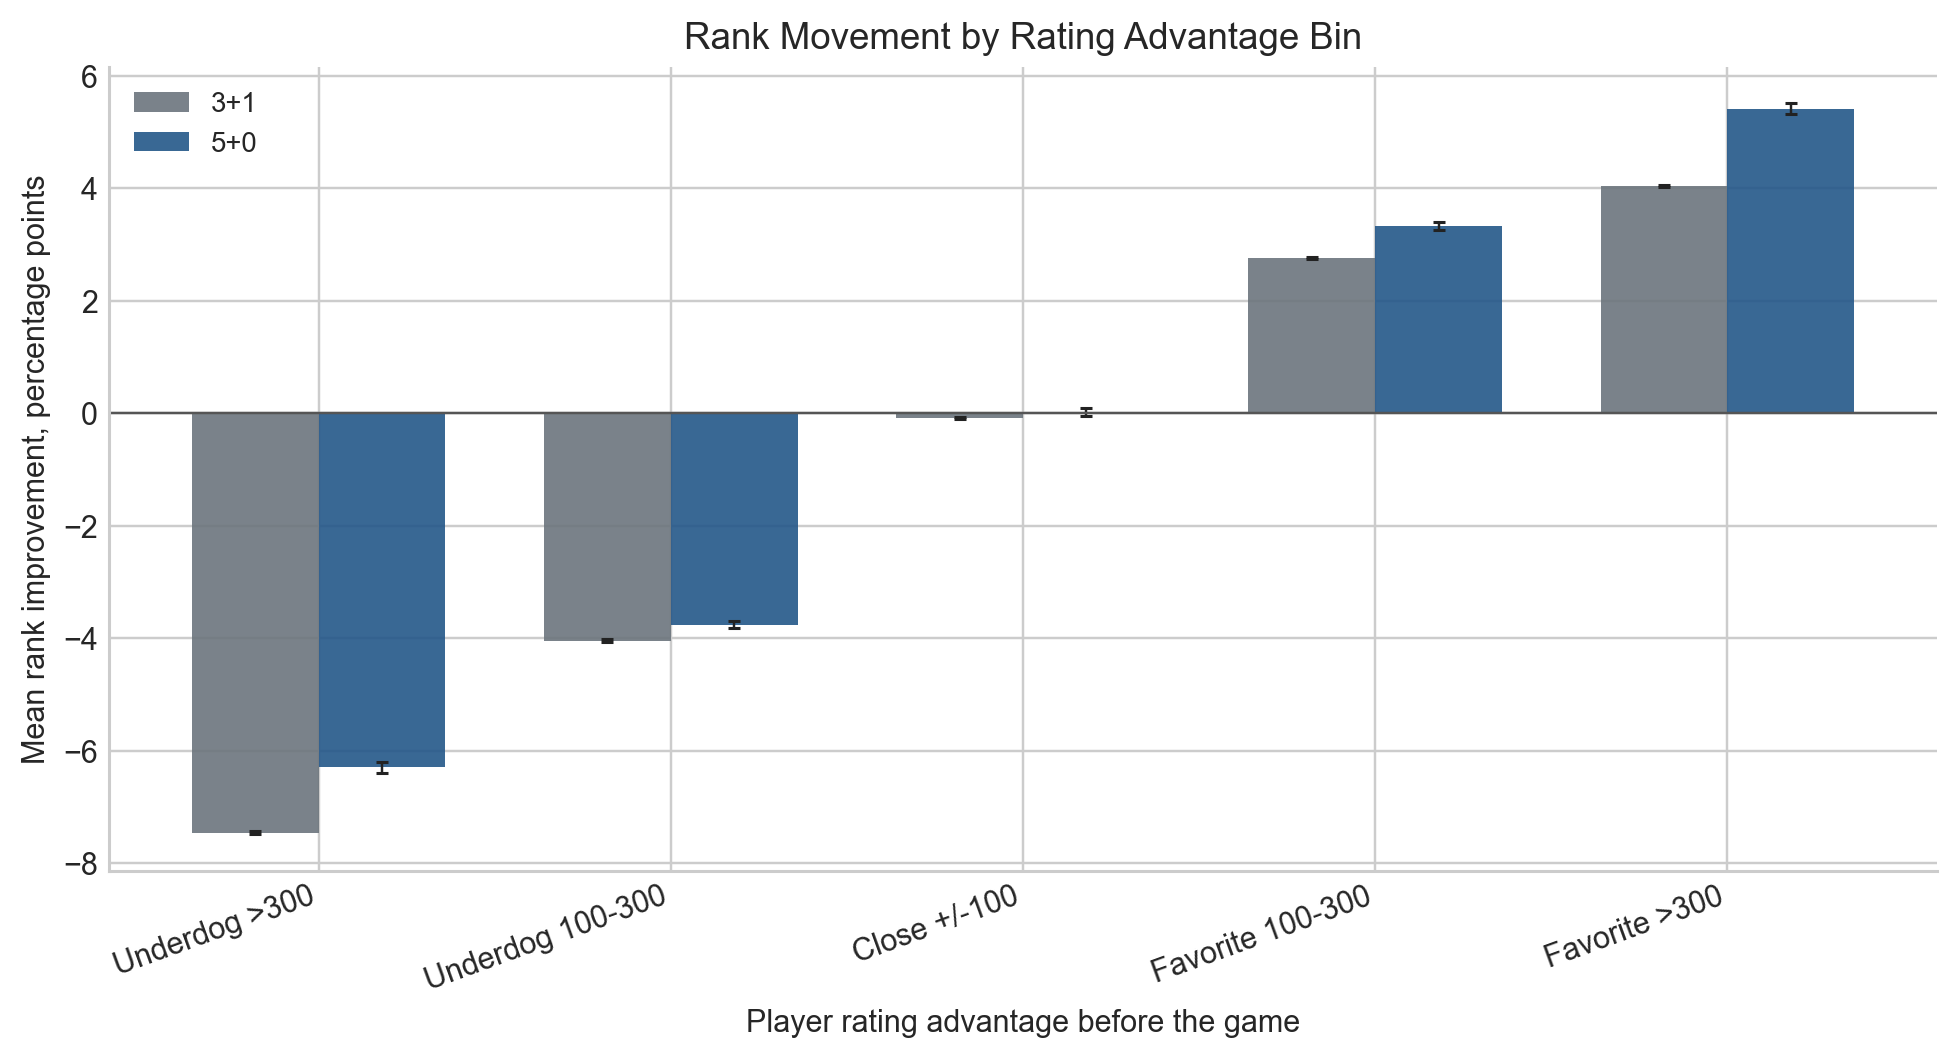
\includegraphics[width=0.90\textwidth]{figures/figure3_rank_movement_by_rating_advantage.png}
\caption{Pre/post rank movement by rating advantage.}
\label{fig:rankmovement}
\end{figure}

These field and pairing results are useful for interpretation. They show that the institutional reform changed both the production environment and the selection environment. The fixed-effect game-level models address conditional performance among observed games; the participation and field-composition results describe who appears in the new environment.

\subsection{Late-Game Error Accumulation}

Figure \ref{fig:stockfish-dashboard} summarizes the move-level mechanism evidence before reporting the individual estimates. The dashboard is useful because the main move-level interpretation does not come from a single coefficient: it comes from phase-specific error profiles, first-blunder timing, rating-bin conversion patterns, and deep conversion/recovery models.

\begin{figure}[H]
\centering
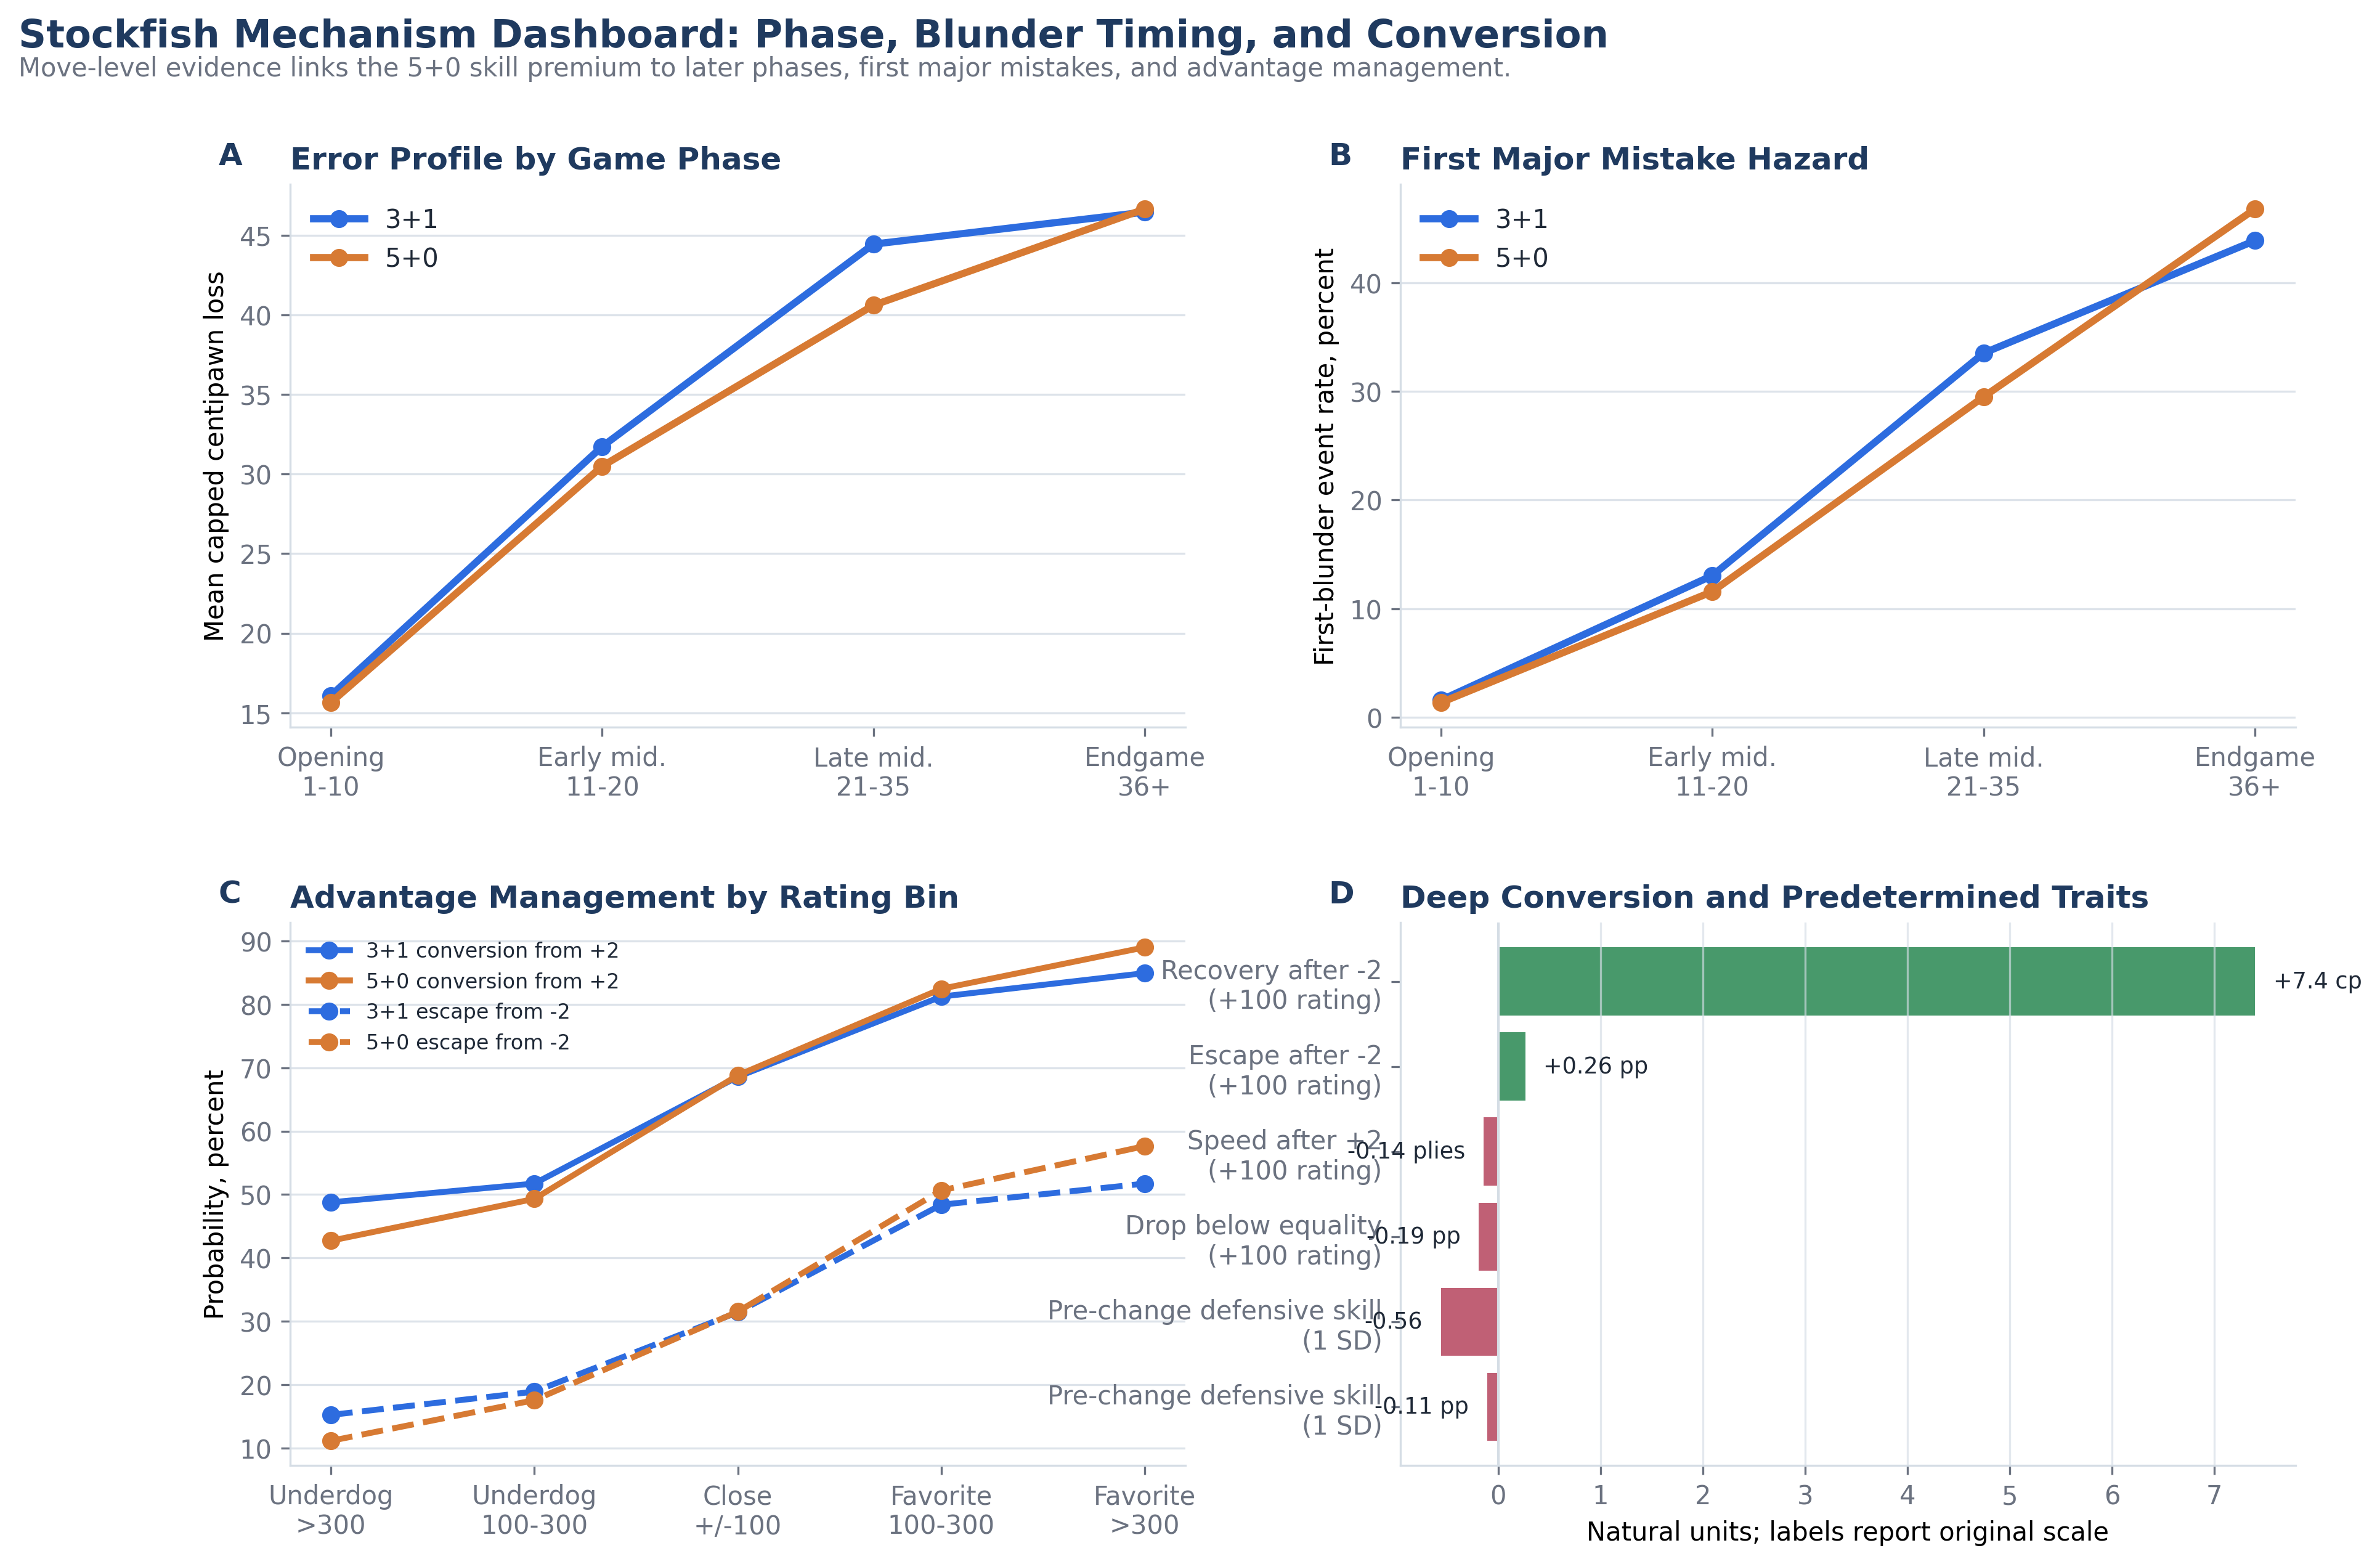
\includegraphics[width=\textwidth]{figures/figure9_stockfish_mechanism_dashboard.png}
\caption{Stockfish mechanism dashboard: phase errors, first-blunder hazard, conversion, and predetermined traits.}
\label{fig:stockfish-dashboard}
\end{figure}

The move-level Stockfish analysis shows that late phases became more costly under 5+0. The main phase model estimates \(\text{Post} \times \text{LatePhase}\) at about 2.06 capped centipawns. The final-ten-ply interaction is about 2.72 capped centipawns. These estimates are small in absolute centipawn terms, but they are estimated over more than 27 million moves and survive fixed effects and clustering. They indicate a systematic shift in where errors occur.

\begin{figure}[H]
\centering
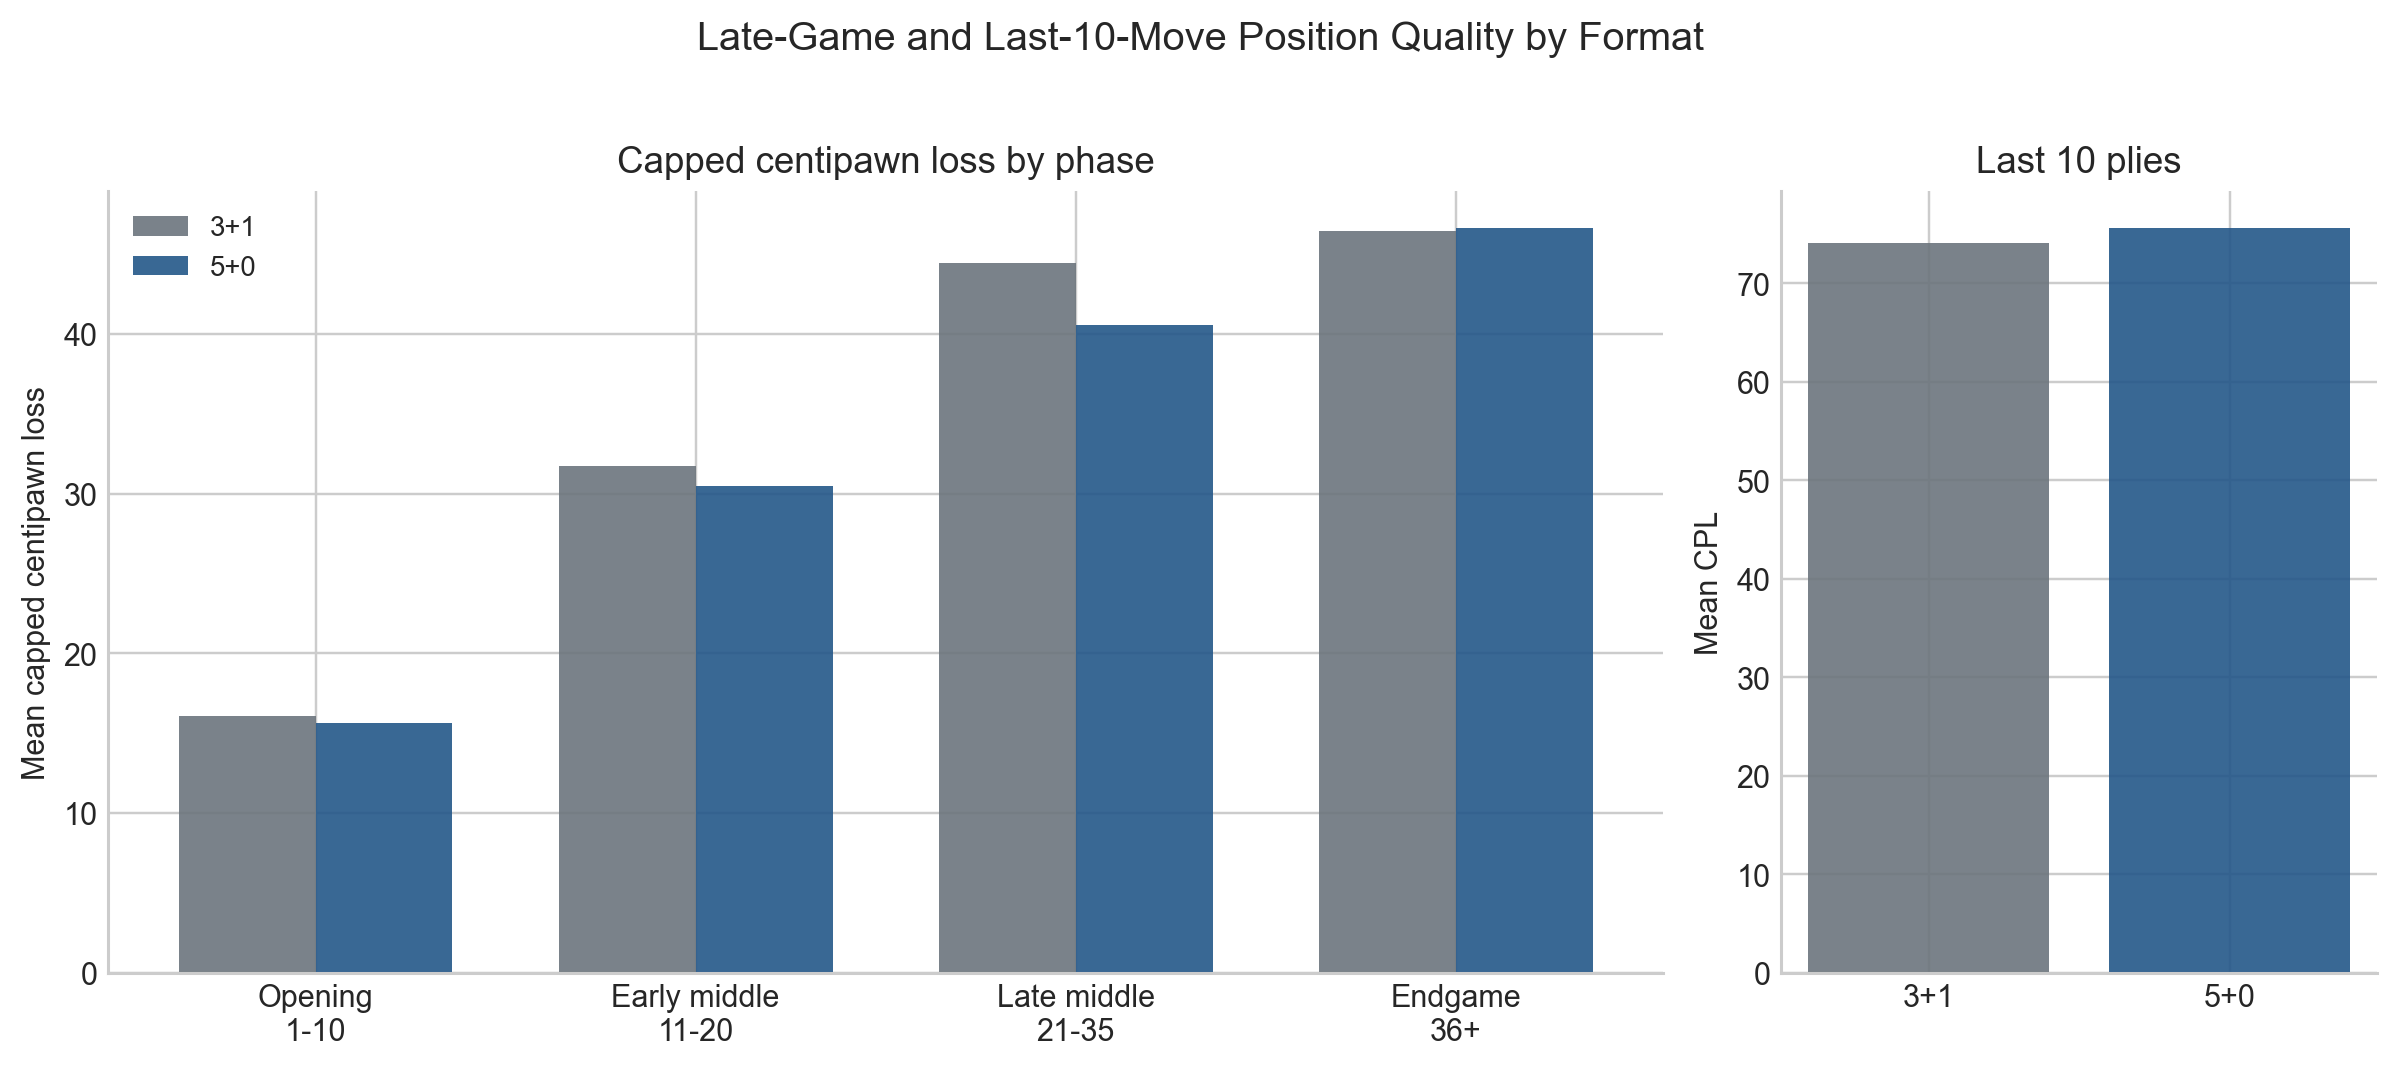
\includegraphics[width=0.90\textwidth]{figures/figure4_phase_last10_cp_loss.png}
\caption{Centipawn loss by phase and final-ten-ply status under 3+1 and 5+0.}
\label{fig:phasecpl}
\end{figure}

First-blunder hazard models show a related phase pattern. The post-change hazard falls in early and late middlegame phases but rises in endgames. The endgame phase interaction is about 0.0289. This phase result is complemented by the direct clock analysis below, which shows that the largest quality penalties are concentrated in severe low-clock states.

\subsection{Critical Positions and First Major Mistakes}

Critical or equal positions are defined as pre-move positions where the mover's engine evaluation is within 100 centipawns of equality. These positions are important because a single error can change the result expectation sharply. The post-change interaction on blunder probability in critical/equal positions is about 0.0020, or 0.20 percentage points. The corresponding capped-centipawn-loss estimate is about 0.75 centipawns.

Age heterogeneity appears in critical positions. The triple interaction \(\text{Post} \times \text{Age10} \times \text{CriticalEqual}\) is about 0.27 capped centipawns, and the triple interaction in blunder probability is positive as well. These estimates suggest that older players face a larger post-change penalty in tactically sensitive equal positions, though the strongest age evidence remains at the player-game level and in first-blunder timing.

First-blunder timing gives another view of how errors are distributed within games. Conditional on having a blunder, a player 10 years older blundered about one-third of a move earlier after the reform. Female players blundered about one move earlier conditional on blundering, but broad female move-level interactions are not robust enough to support a general female-specific deterioration story. The no-blunder-game probability by age is weaker after multiple-testing adjustment, so first-blunder timing is the preferred error-timing result.

\subsection{Clock-Time Mechanisms}

The clock data refine the interpretation of the move-level results. The simple story would be that 5+0 mechanically creates more time pressure. This is not what the data show. Because the new format gives each player five initial minutes instead of three, ordinary low-clock exposure actually falls. The share of moves started with 10 seconds or less falls from about 10.0\% before the reform to 3.8\% after the reform, and the mean final clock rises from 33.3 seconds to 64.7 seconds. Figure \ref{fig:clock-exposure-insurance} visualizes this shift. The important change is therefore not the average amount of time pressure, but the technology of severe time pressure. In 3+1, a player who reaches a very low clock can sometimes rebuild time through the one-second increment. In 5+0, recovery is essentially impossible.

\begin{figure}[H]
\centering
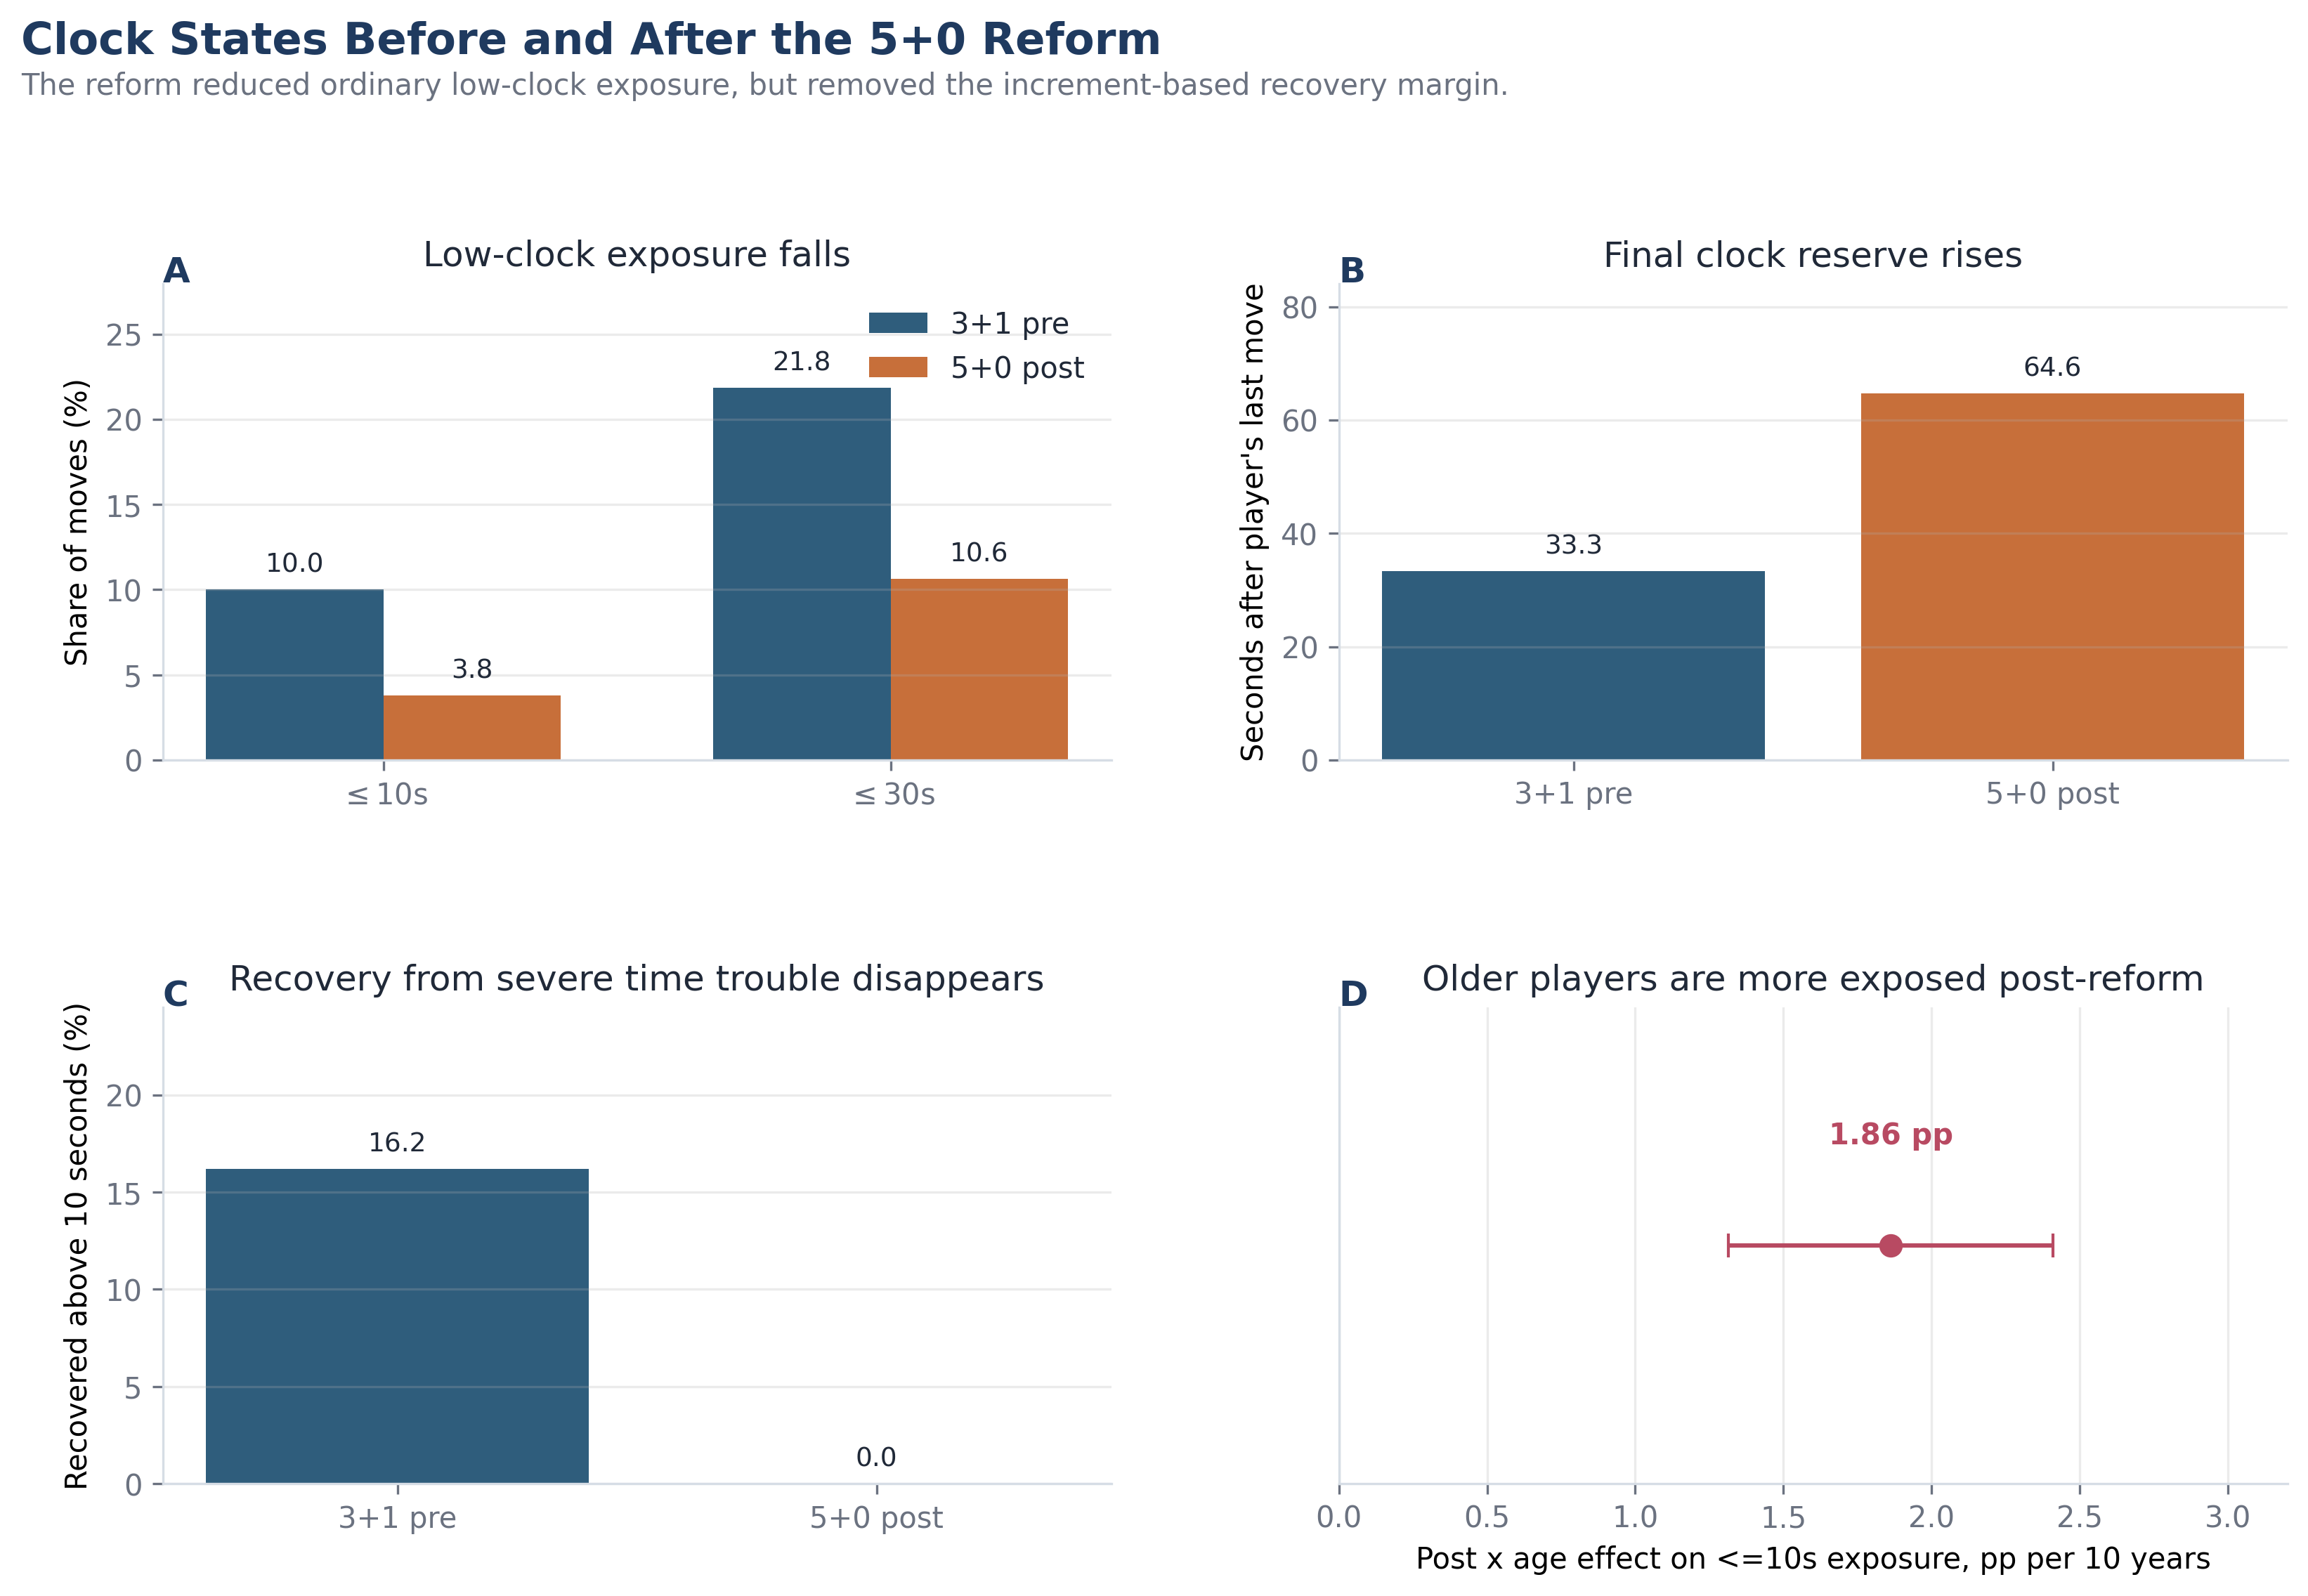
\includegraphics[width=\textwidth]{figures/figure12_clock_exposure_insurance.png}
\caption{Clock states before and after the reform: low-clock exposure, final clock reserve, low-clock recovery, and age heterogeneity.}
\label{fig:clock-exposure-insurance}
\end{figure}

\begin{table}[H]
\centering
\caption{Robust Clock-Time Mechanisms}
\label{tab:clock-mechanisms}
\small
\begin{adjustbox}{max width=\textwidth}
\begin{tabular}{p{0.24\textwidth}p{0.25\textwidth}p{0.18\textwidth}p{0.24\textwidth}}
\toprule
Mechanism & Main estimate & Significance & Interpretation \\
\midrule
Lower ordinary low-clock exposure & Post effect on share of moves starting with \(\leq 10\) seconds: \(-0.0734\) & \(p<0.001\) & Players reach very low clock less often because 5+0 starts with a larger time budget. \\
Higher cost of severe time trouble & Post interaction for \(\leq 10\)-second exposure: \(+19.82\) capped centipawns; exact bin interactions: \(+14.87\) cp for 5--10s and \(+29.15\) cp for 0--5s & \(p<0.001\) & Once severe time trouble occurs, move quality deteriorates much more under 5+0. \\
Loss of increment insurance & Post effect on recovery above 10 seconds after entering \(\leq 10\) seconds: \(-0.1648\) & \(p<0.001\) & Under 3+1 some players rebuild time; under 5+0 this margin essentially disappears. \\
Clock weakness and conversion & Own low clock at first winning position: post penalty about \(-0.29\); opponent low clock at first winning position: post gain about \(+0.10\); opponent low clock when worse: post escape gain about \(+0.30\) & \(p<0.001\) & Low own clock makes winning positions harder to convert, while opponent clock weakness becomes a valuable practical resource. \\
Age and clock adaptation & Post-by-age effect on \(\leq 10\)-second exposure: \(+0.0186\) per 10 years & \(p<0.001\) & Older players are relatively more exposed to very low-clock states after the reform. \\
\bottomrule
\end{tabular}
\end{adjustbox}
\end{table}

These estimates support a specific mechanism. The no-increment format does not simply make every move faster or noisier. It reduces the frequency of ordinary low-clock states but increases the marginal cost of reaching extreme time trouble. The exact move-bin regressions show that the post-change penalty is small or negative in moderate clock bins, but rises sharply below 10 seconds. Event-time models around the first low-clock crossing lead to the same conclusion: first crossing below 30 seconds does not generate a persistent post-change error cascade, while first crossing below 10 seconds does. Figure \ref{fig:clock-panic-conversion} shows both the panic-threshold pattern and the conversion role of own and opponent low-clock states.

\begin{figure}[H]
\centering
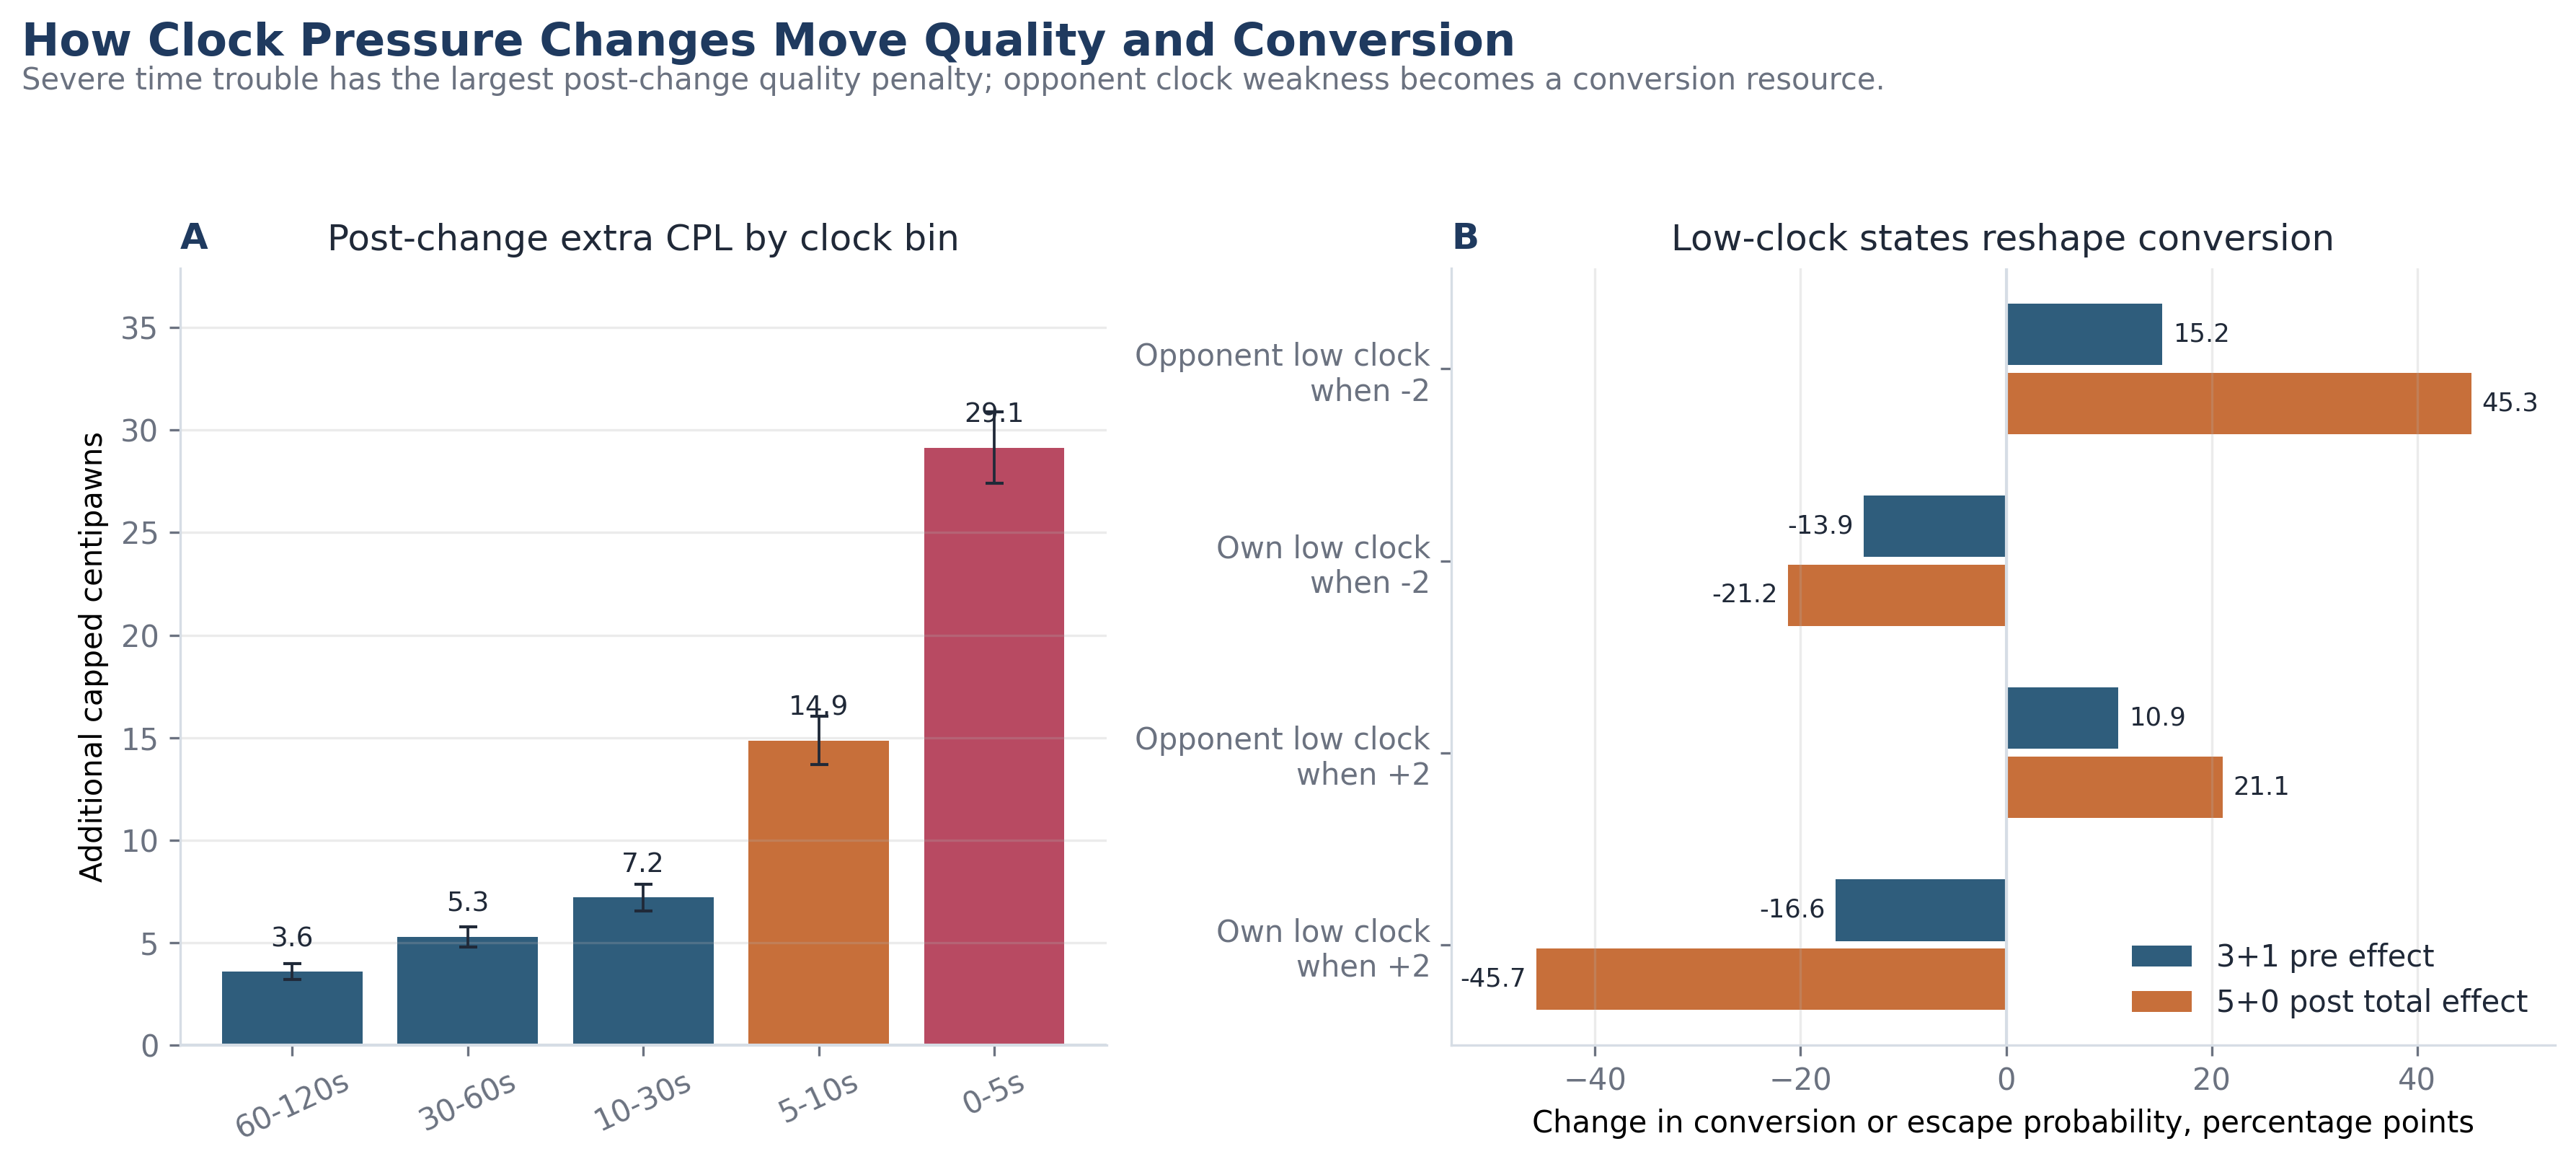
\includegraphics[width=\textwidth]{figures/figure13_clock_panic_conversion.png}
\caption{Clock pressure mechanisms: post-change centipawn-loss penalties by clock bin and low-clock effects on conversion or defensive escape.}
\label{fig:clock-panic-conversion}
\end{figure}

Clock states also change conversion technology. When a player first reaches a winning engine position while personally below 10 seconds, conversion becomes much harder after the reform. Conversely, if the opponent is already below 10 seconds when the player reaches a winning or losing engine state, the player converts or escapes much more often. This result connects the clock analysis to the main skill-premium result: under 5+0, objective board advantage, engine-measured accuracy, and clock capital jointly determine whether advantages become points.

\subsection{Conversion From Winning Positions and Defensive Recovery}

The conversion results connect the game-level skill premium to concrete move-level mechanisms. Winning positions are defined as positions where the player reached at least +200 centipawns from the engine's perspective at least ten plies before the game ended. A stronger rating advantage increased post-change conversion from winning positions by about 0.33 percentage points per 100 rating points. The defensive escape model is also positive: a 100-point rating advantage increased post-change escape from losing positions by about 0.40 percentage points.

\begin{table}[H]
\centering
\caption{Move-Level and Conversion Mechanisms}
\label{tab:move-mechanisms}
\begin{adjustbox}{max width=\textwidth}
\begin{tabular}{llrrrl}
\toprule
Result & Outcome & Estimate & SE & p-value & Unit \\
\midrule
Late phase error & Capped CPL & 2.0566 & 0.3245 & \(<0.001\) & Endgame, fullmove 36+ \\
Last-10-ply error & Capped CPL & 2.7231 & 0.4975 & \(<0.001\) & Final 10 plies \\
Critical/equal blunder & Blunder probability & 0.0020 & 0.0003 & \(<0.001\) & \(|eval|<100\) cp \\
Critical/equal CPL & Capped CPL & 0.7466 & 0.1795 & \(<0.001\) & \(|eval|<100\) cp \\
Winning conversion & Converted +2 & 0.0033 & 0.0007 & \(<0.001\) & Per +100 rating advantage \\
Defensive escape & Escaped -2 & 0.0040 & 0.0008 & \(<0.001\) & Per +100 rating advantage \\
Conversion speed & Plies to conversion & -0.1425 & 0.0302 & \(<0.001\) & Per +100 rating advantage \\
Recovery after -2 & Recovery probability & 0.0026 & 0.0006 & \(<0.001\) & Per +100 rating advantage \\
First blunder by age & First blunder move & -0.3315 & 0.0735 & \(<0.001\) & Per +10 years \\
\bottomrule
\end{tabular}
\end{adjustbox}
\end{table}

The deeper conversion results are especially informative. After reaching +2, stronger players converted faster under 5+0: the estimate is -0.1425 plies per 100 rating points. They were also less likely to drop the position back below equality, with an estimate of -0.0019 per 100 rating points. After reaching -2, stronger players recovered more, gaining about 7.4 centipawns more in the recovery measure and increasing recovery probability by about 0.26 percentage points per 100 rating points.

\begin{figure}[H]
\centering
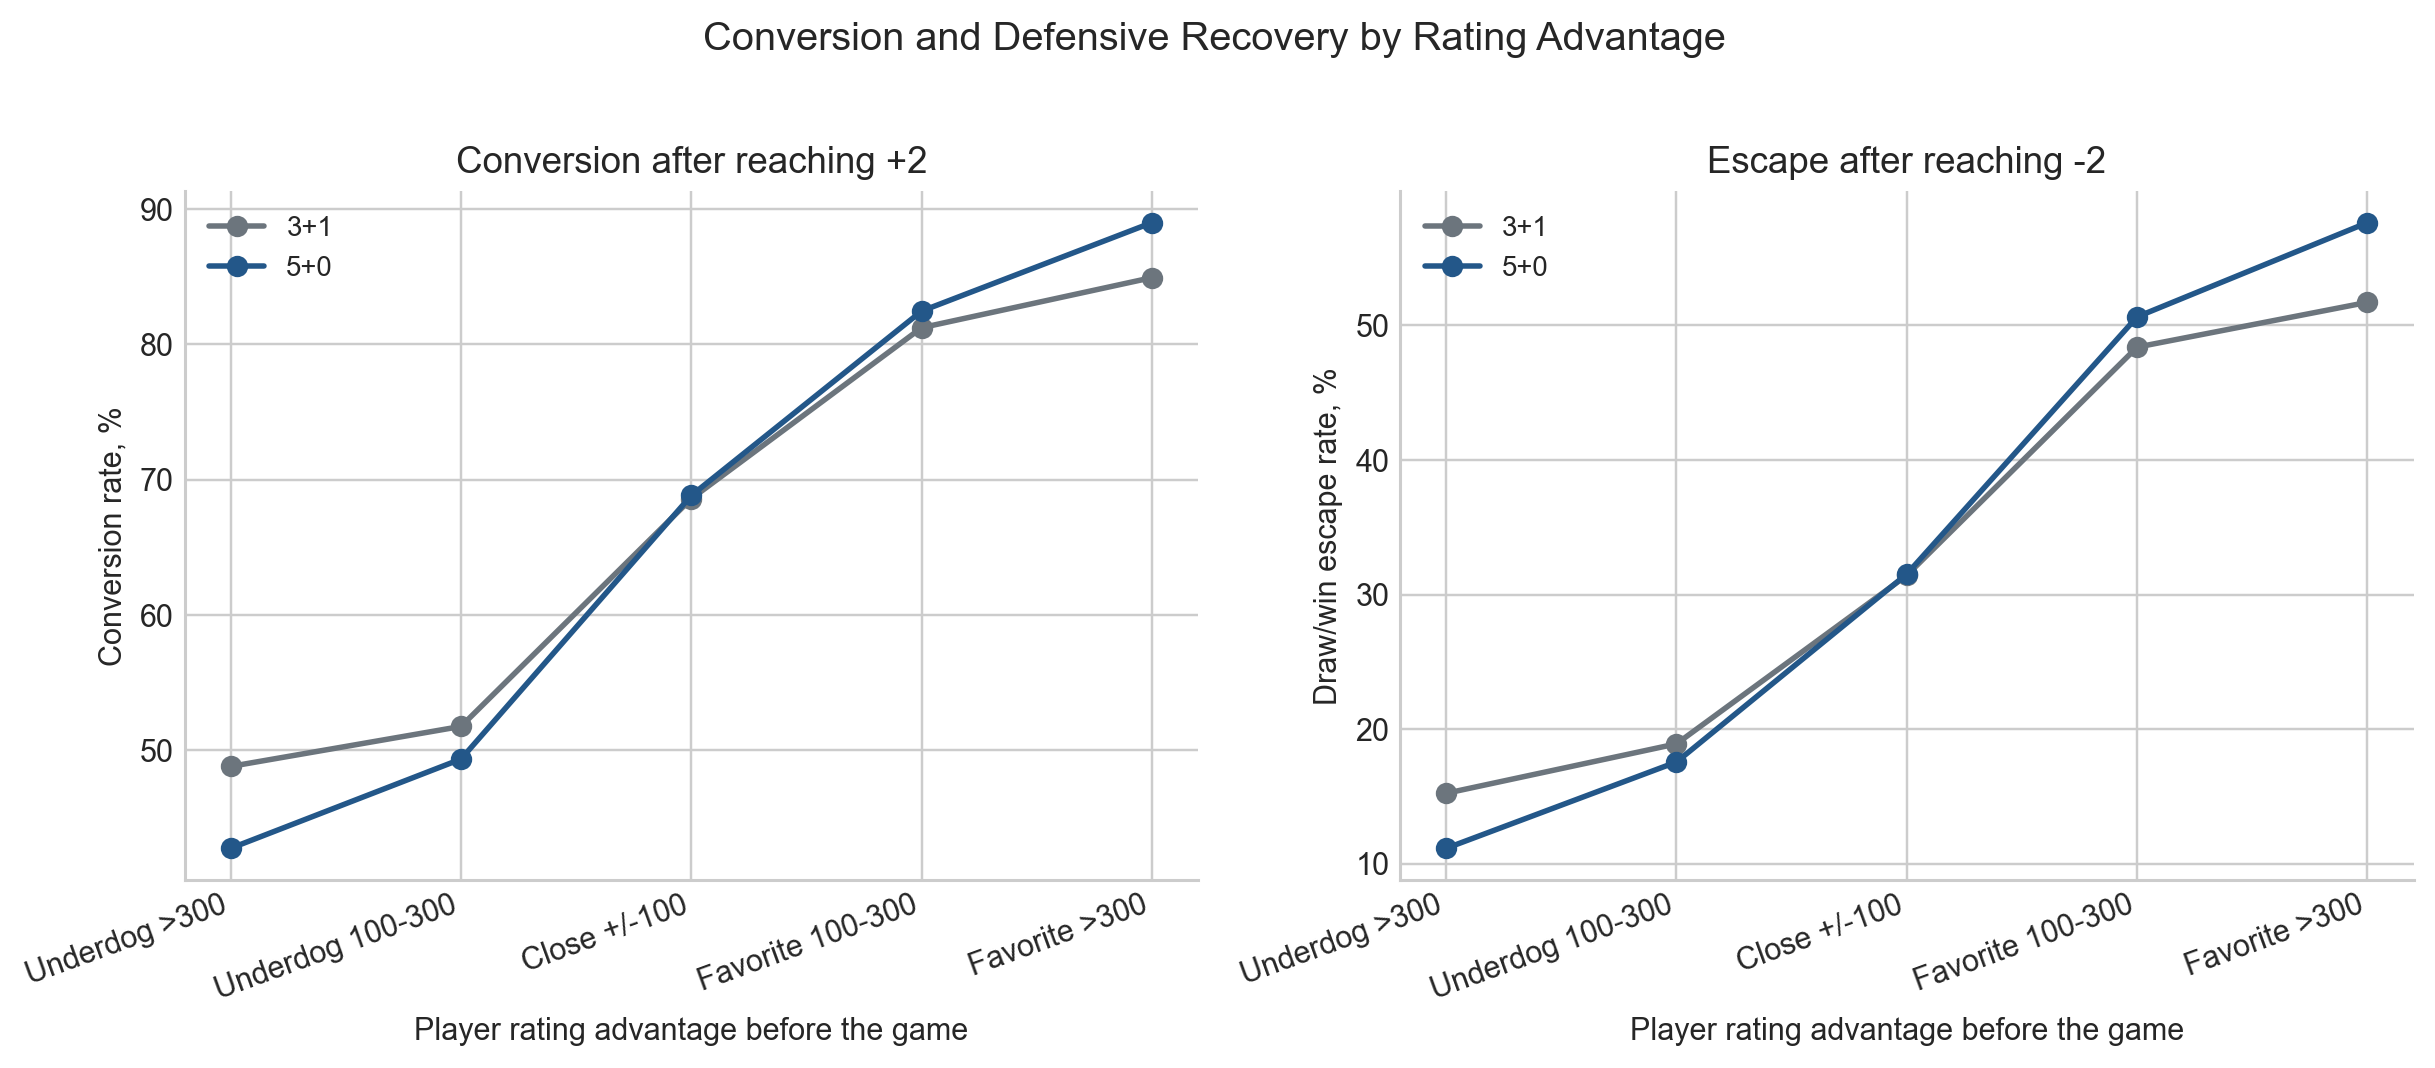
\includegraphics[width=0.90\textwidth]{figures/figure5_conversion_recovery_by_rating_advantage.png}
\caption{Conversion from +2 and recovery from -2 by rating advantage.}
\label{fig:conversion}
\end{figure}

Together these results show that the post-change skill premium is not just a rating-table artifact. It appears in advantage management. Stronger players convert winning positions more efficiently, lose fewer advantages, and recover more from worse positions under the no-increment format.

\subsection{Complexity and Predetermined Skill Traits}

The complexity results are nuanced. The data do not show that all complex positions became uniformly worse under 5+0. Instead, complexity moderates who benefits. The interaction \(\text{Post} \times \text{ComplexityIndex}\) in capped centipawn loss is negative, while the triple interaction \(\text{Post} \times \text{Age10} \times \text{ComplexityIndex}\) is positive. This means that complex positions were not simply worse for everyone, but older players faced relatively higher post-change losses in complex settings.

Predetermined pre-change traits support the same interpretation. Players with stronger pre-change defensive skill had lower post-change blunder rates and lower capped centipawn loss. Players with greater pre-change complexity tolerance also had lower post-change error rates. The estimates are around -0.0011 for blunder rate and -0.56 capped centipawns for defensive skill, and around -0.0008 for blunder rate and -0.54 capped centipawns for complexity tolerance. These are not enormous effects, but they are conceptually valuable because the traits are measured before the rule change.

\subsection{Playing Style}
\label{sec:playing-style}

The style analysis is deliberately based on pre-change behavior, so it can be interpreted as heterogeneity by predetermined player type rather than as a mechanical consequence of the new format. The analysis uses two complementary style measures. The first is an interpretable feature approach based on pre-change Stockfish and move variables. The second is a neural style-embedding approach that learns player representations directly from pre-change move sequences.

The interpretable approach centers on four indexes: clean style, chaos creation, self-risk, and practical chaos. The strongest econometric result is the post-change penalty for chaos-style profiles. In several player-game result models, a one-standard-deviation increase in pre-change chaos style is associated with about 1.0 to 1.4 percentage points lower post-change score share. This is a relative-payoff result, not a statement that such players became objectively worse in every dimension. It means that, conditional on the empirical specification, players with more chaotic pre-change profiles did not receive a larger score premium from the switch to 5+0.

Figure \ref{fig:style-feature-pca} visualizes how the interpretable and neural approaches relate to each other. The axes are the first two principal components of standardized pre-change interpretable features, while the colors are the five clusters learned from the neural contrastive style embeddings. Thus the figure should not be read as a PCA of the neural embedding space. It shows that the neural clusters line up with transparent chess dimensions: PC1 explains about 64.8 percent of the interpretable-feature variance and mainly separates clean, low-error players from volatile and error-prone players; PC2 explains about 11.0 percent and contrasts tactical activity with longer, quieter games. An interactive version of the style analysis, including searchable player-level visualizations, is available at \url{https://eli-sumernikov-master-thesis-styles.netlify.app}.

\begin{figure}[H]
\centering
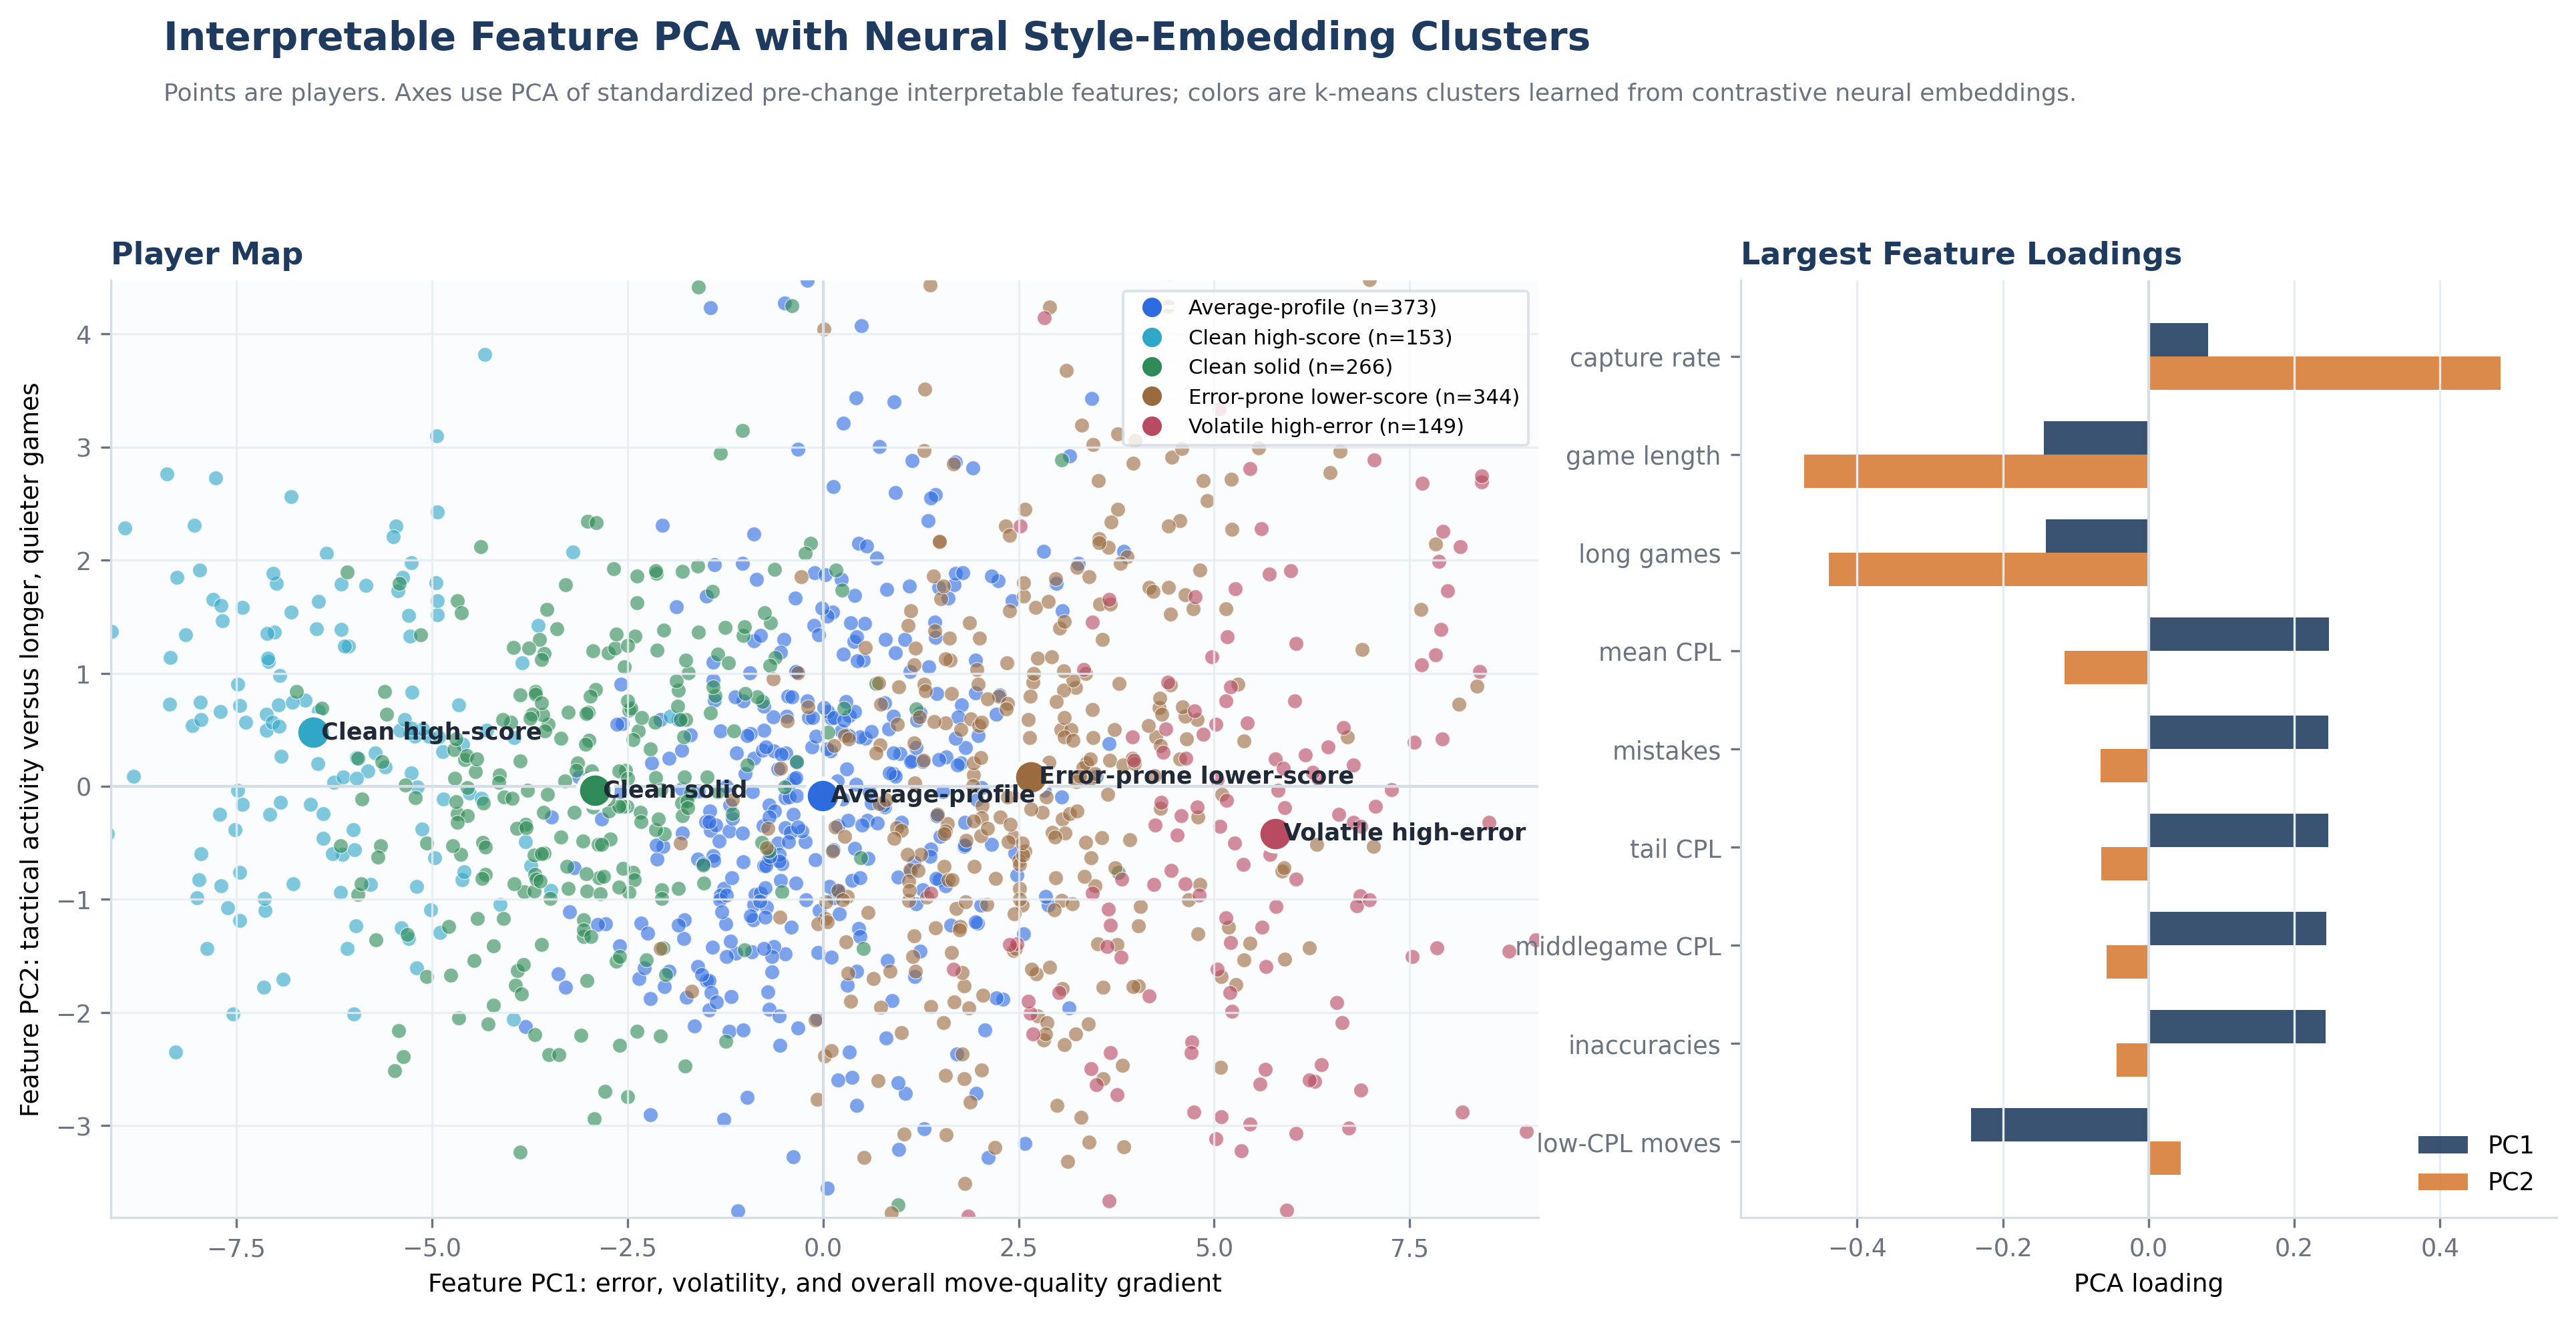
\includegraphics[width=\textwidth]{figures/figure11_interpretable_style_feature_pca.png}
\caption{Interpretable-feature PCA with neural style-embedding clusters. The axes are principal components of pre-change interpretable style features; the colors are clusters learned from contrastive neural player embeddings.}
\label{fig:style-feature-pca}
\end{figure}

\begin{table}[H]
\centering
\caption{Style Index Interactions}
\label{tab:style}
\begin{adjustbox}{max width=\textwidth}
\begin{tabular}{llrrrl}
\toprule
Model & Term & Estimate & SE & p-value & Unit \\
\midrule
Heavy-underdog result & Post \(\times\) chaos index & -0.0139 & 0.0053 & 0.009 & Per 1 SD chaos \\
Favorites-only result & Post \(\times\) chaos index & -0.0131 & 0.0056 & 0.020 & Per 1 SD chaos \\
Underdog triple model & Post \(\times\) chaos index & -0.0127 & 0.0057 & 0.025 & Per 1 SD chaos \\
Online-capital controls & Post \(\times\) chaos index & -0.0109 & 0.0051 & 0.034 & Per 1 SD chaos \\
Result over expected & Post \(\times\) chaos index & -0.0099 & 0.0047 & 0.035 & Per 1 SD chaos \\
Practical chaos model & Post \(\times\) practical chaos & -0.0107 & 0.0049 & 0.031 & Per 1 SD practical chaos \\
\bottomrule
\end{tabular}
\end{adjustbox}
\end{table}

This result rejects a plausible alternative story in which no-increment chess simply rewards practical chaos. The evidence points toward clean conversion and defensive stability as safer profiles after the reform. At the same time, the neural cluster results below show that the reform did not help only one narrow style group. All five neural style clusters improved their raw average accuracy after the switch; the difference is that chaotic profiles did not gain a relative score premium.

The neural style-embedding model is trained on player-game sequences from pre-change games only. Eligibility is defined using the full player-game panel: a player must have at least 100 total games and must appear both before and after the September 2025 rule change. This gives 1,295 eligible players in metadata, of whom 1,285 are matched to pre-change style features and usable move sequences. The sequence builder scans 805,256 PGN games, selects 519,945 pre-change games for eligible players, and writes 602,033 player-game sequences. To focus on style rather than memorized theory or forced late-game residues, the first 10 full moves and the last 10 plies are excluded. Sequences shorter than 12 moves are dropped and longer sequences are capped at 80 moves.

Each move token contains nine categorical fields: moved piece, origin square, destination square, capture indicator, check indicator, phase, binned centipawn loss, binned pre-move evaluation from the mover's perspective, and move-number bin. These tokens are passed through field embeddings, a feed-forward input layer, and a bidirectional GRU. The final hidden states are projected to a 64-dimensional normalized game embedding. The model is trained with a supervised contrastive loss: in each batch, two games from the same player are positives, while games from other players are negatives. The implementation uses 64 players per batch, two games per player, temperature 0.10, 10 percent within-player validation, and early stopping. Player embeddings are the averages of their pre-change game embeddings.

The averaged player embeddings are clustered with \(k\)-means. A grid over \(k=3,\ldots,8\) gives silhouette scores around 0.49 to 0.52; the five-cluster solution has a silhouette score of 0.497 and provides the most useful substantive granularity. The five clusters correspond to clean high-score players, clean solid players, average-profile players, error-prone lower-score players, and volatile high-error players.

\begin{figure}[H]
\centering
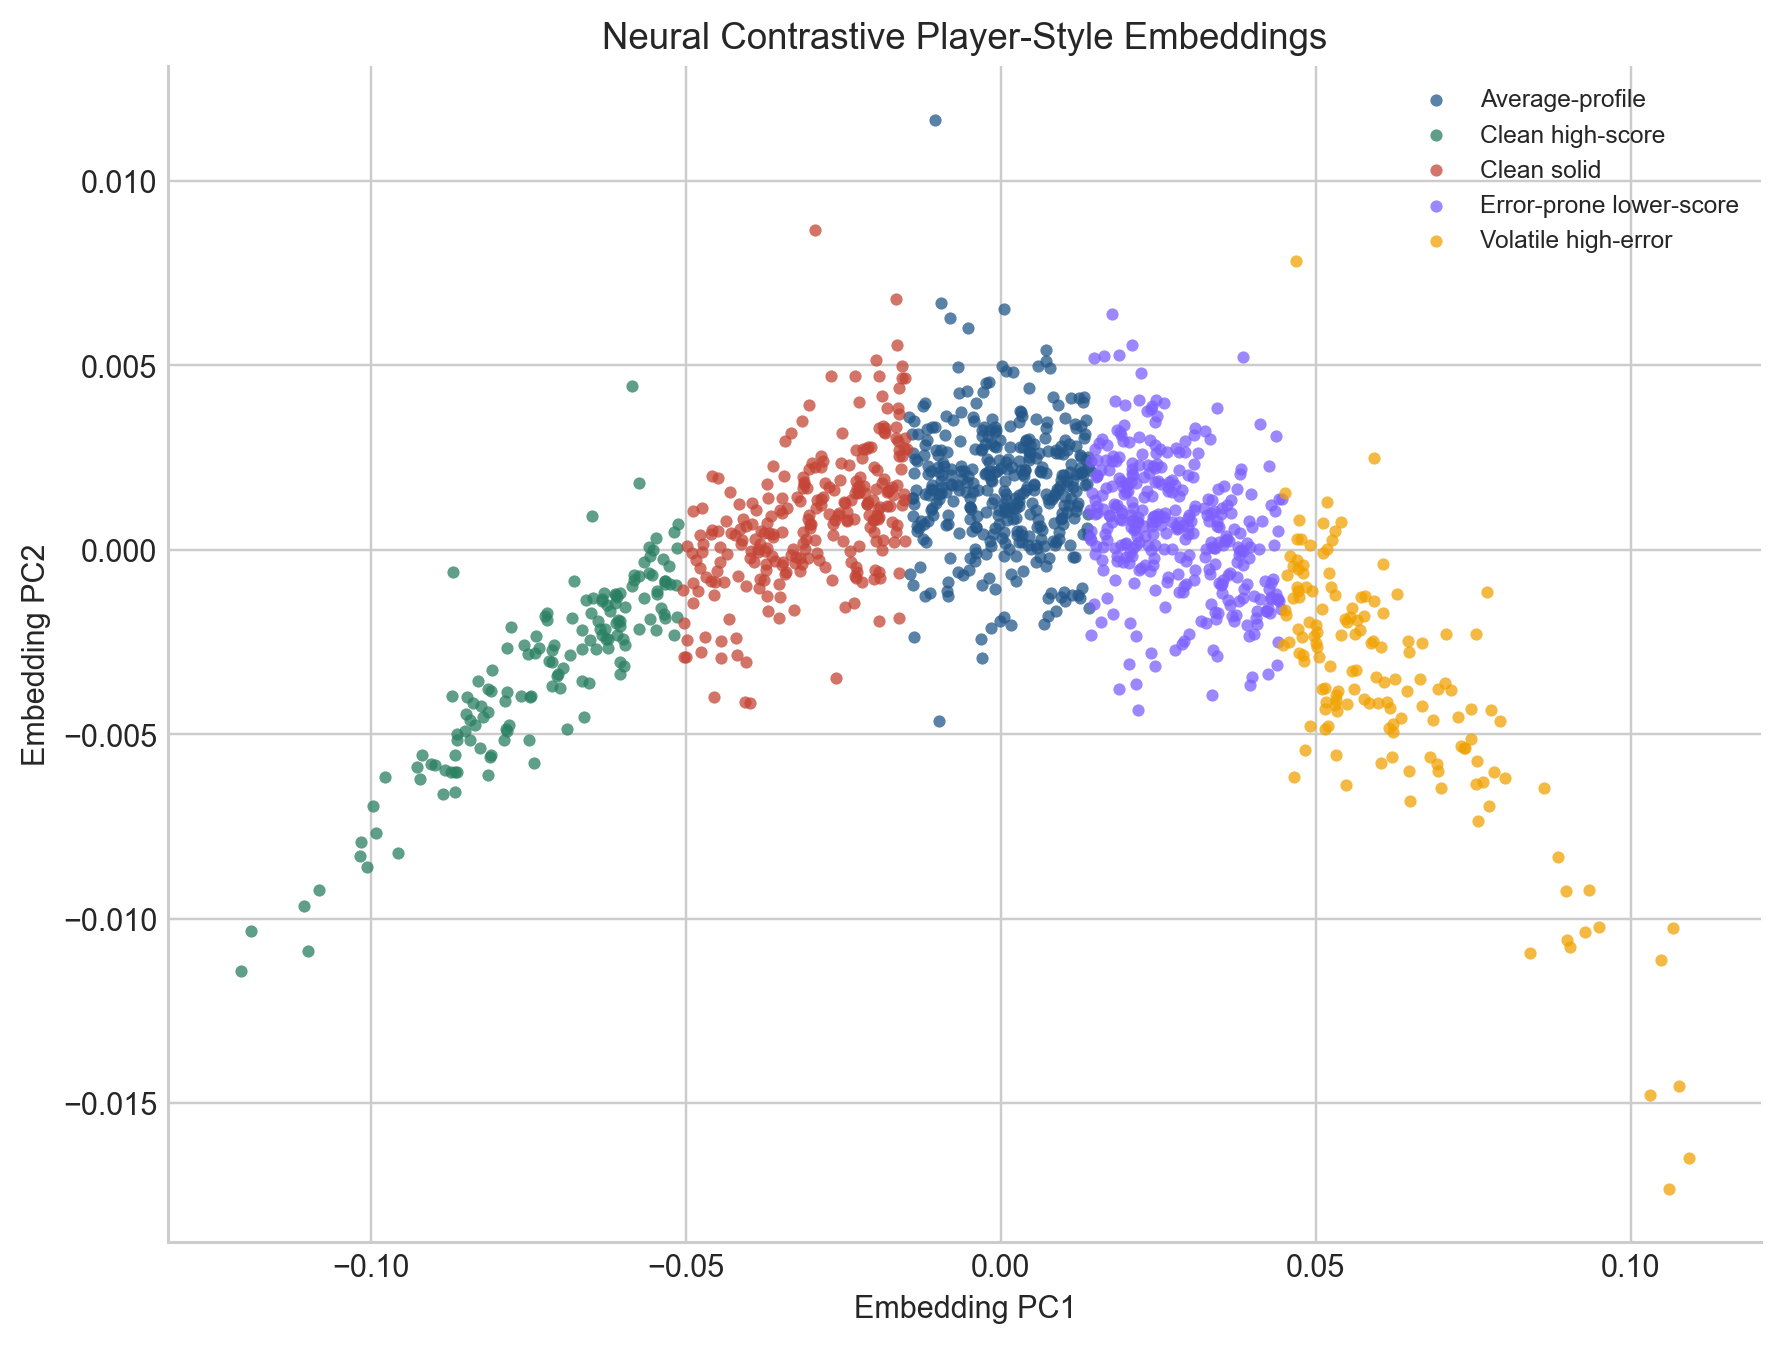
\includegraphics[width=0.85\textwidth]{figures/figure6_neural_style_cluster_map_static.png}
\caption{PCA of learned contrastive player embeddings. The plot shows the same five neural clusters in the two-dimensional projection of the 64-dimensional embedding space.}
\label{fig:neural-style}
\end{figure}

Table \ref{tab:neural-style-clusters} summarizes the cluster profiles. The clean high-score cluster is the strongest group ex ante: its average pre-change score share is 0.692, its mean centipawn loss is 28.4, and 57.3 percent of its pre-change games contain no player blunder. The clean solid cluster is less dominant in results but still low-error, with mean centipawn loss of 32.6 and a no-blunder-game rate of 46.0 percent. The average-profile cluster sits near the sample center. The error-prone lower-score and volatile high-error clusters have substantially higher centipawn loss, higher blunder rates, and lower pre-change score shares.

\begin{table}[H]
\centering
\caption{Neural Style-Embedding Cluster Profiles}
\label{tab:neural-style-clusters}
\begin{adjustbox}{max width=\textwidth}
\begin{tabular}{lrrrrrr}
\toprule
Cluster label & Players & Pre result & Mean CPL & No-blunder games & Accuracy delta & Result delta \\
\midrule
Clean high-score & 153 & 0.692 & 28.38 & 0.573 & 0.616 & -0.0216 \\
Clean solid & 266 & 0.579 & 32.60 & 0.460 & 0.752 & -0.0217 \\
Average-profile & 373 & 0.496 & 36.07 & 0.387 & 0.801 & -0.0176 \\
Error-prone lower-score & 344 & 0.421 & 39.38 & 0.336 & 0.711 & -0.0197 \\
Volatile high-error & 149 & 0.355 & 43.78 & 0.266 & 0.653 & -0.0176 \\
\bottomrule
\end{tabular}
\end{adjustbox}
\end{table}

The important result is that all five neural style clusters show positive raw accuracy changes after the reform, from about +0.62 to +0.80 Chess.com accuracy points on equal-player averages. This is informative because it rules out a simple story in which only clean or elite styles adjusted to the new time control. The broad accuracy improvement is consistent with the extra two minutes of initial time improving average move quality. The score-share deltas are small and mostly negative across clusters, which should not be interpreted as a causal style loss because the post-change tournament field, participation composition, and schedule changed at the same time. The causal style evidence therefore comes from the fixed-effect style-index regressions, while the neural embedding model contributes two things: it shows that pre-change move sequences contain stable player-style information, and it shows that the move-quality improvement after 5+0 was broad across learned style groups.

\subsection{Synthesis}

The robust results describe a coherent pattern. First, 5+0 increased returns to skill rather than randomness: rating advantages and accuracy advantages became more valuable. Second, the mechanism is conversion under constraint: stronger players converted advantages faster, lost fewer winning positions, recovered better from inferior positions, and avoided the style penalty associated with chaos. Third, the clock evidence shows why the constraint changed. Players had more initial time and less ordinary low-clock exposure, but severe time trouble became much more dangerous because the increment no longer insured recovery. Fourth, adaptability is heterogeneous: younger players, online specialists, and players with pre-change defensive or complexity-tolerance traits appear better positioned for the new format. Fifth, the tournament itself changed through selection: old late-slot regulars were hurt mainly through participation and completion, not through lower per-game move quality.
